\ifdefined\XeTeXrevision\else\pdfoutput=1\fi
\documentclass[11pt]{article}
\usepackage[margin=1in]{geometry}
\usepackage{graphicx,booktabs,amsmath,amssymb,caption,enumitem,xcolor,hyperref,microtype,longtable,array}
\usepackage[section]{placeins}
\hypersetup{colorlinks=true,linkcolor=blue!55!black,citecolor=blue!55!black,urlcolor=blue!55!black,
pdftitle={Conditional LoRA Bridges: Separating Adaptation Capacity from Sensor Conditioning},pdfauthor={Franci Penov}}
\graphicspath{{figures/}}
\setlength{\emergencystretch}{2em}
\newcommand{\RevisionDate}{September 07, 2026 --- revision 2}

\title{Conditional LoRA Bridges:\\Separating Adaptation Capacity from Sensor Conditioning}
\author{Franci Penov\\kortexa.ai\\\texttt{francip@kortexa.ai}}
\date{\RevisionDate}
\begin{document}
\maketitle
\begin{abstract}
A hypernetwork can condition a frozen language model by generating low-rank weight updates from sensor features. The same bridge also adds trainable capacity, so improved text likelihood alone is an ambiguous indicator of sensor use. We separate these effects with independently sampled text, paired category probes, and a separately trained instruction-generation cohort. The study retains the original 33.6M host and adds pinned 230M and 0.8B hosts, with matched constant, shuffled, random, static-adapter, and frozen references. Under independent sampling, 9 of 9 true-minus-constant BPB intervals include zero. This does not establish equivalence or extend to all paired likelihood objectives. Full held-out populations, grouped intervals, and same-checkpoint interventions assess conditioning. Numerical training failures affected 25 of the 411 declared trials; the corresponding endpoint estimates are unavailable. Mini reaches macro rank-1 accuracy 0.461 on audio, 0.582 on vision; Qwen 0.8B reaches macro rank-1 accuracy 0.838 on IMU, 0.421 on audio, 0.451 on vision. On held-out templates, Qwen's IMU joint label and sentence success is 0.838 and 0.689; sensor replacement tests their input dependence. Success on both reversed rule mappings is 0.005. Audio generation varies substantially across seeds. We report training-budget trajectories, effective-update variation, three composition operators, and measured bridge costs. The dense output head grows with adapted dimensions, and workstation results do not establish edge efficiency. Audio evidence is limited by the original encoder's use of held-out inputs in normalization. Claims about likelihood, input prefixes, and generation are scoped to the tested objectives and interfaces; the complete evidence and per-paper reproduction code accompany the revision.

\end{abstract}

\section{Introduction}
A frozen language model can receive sensor information through changes to its
effective weights. A hypernetwork can map an external encoder's features to
low-rank updates, while both the encoder and the language model remain frozen.
This interface is modular, but its success must be measured carefully. A bridge
also adds trainable parameters. Better text likelihood can therefore reflect
ordinary text adaptation even when changing the sensor input is unnecessary.

We study this distinction with three separately trained cohorts. Cohort U uses
independently sampled text and sensor features. Cohort P uses paired sensor and
category examples. Cohort G uses paired sensors, instructions, and target
responses. U tests text adaptation under a deliberately unpaired objective; P
tests closed-set label ranking; G tests bounded sensor-dependent generation.
The cohorts share an interface and controls, but their trained checkpoints and
supervision differ. In addition, we apply several measurements and input
interventions to each saved checkpoint. This avoids attributing a result from a
task-trained bridge to a bridge trained only on unpaired text.

The distinction concerns the data and target distribution, not an intrinsic
defect in likelihood metrics. If a sensor and its target text are paired,
conditioning can reduce text cross-entropy. In U, there is no designed semantic
alignment for sensor shuffling to break. A constant-feature bridge tests whether
variable sensor input is necessary for the observed improvement under that
specific protocol. A small or statistically uncertain difference between true
and constant features is not a proof of equivalence.

This revision extends the original mini-model study with two pinned larger
hosts, full held-out task populations, seed and cluster uncertainty, vision
probes, generation tests, effective-update diagnostics, and measured resource
costs. The contribution is a controlled account of when this interface carries
useful sensor information, what its controls establish, and where its cost or
behavior limits its use. It is not a general multimodal assistant benchmark.

\section{Interface and controls}
\label{sec:method}
\paragraph{Conditional low-rank updates.}
Let $f=e(s)$ be the feature vector of a frozen sensor encoder. The bridge
$h_\theta$ produces $w(f)\in\mathbb{R}^{D}$, partitioned into factors
$A_i(f)\in\mathbb{R}^{d_i^{\rm in}\times r}$ and
$B_i(f)\in\mathbb{R}^{r\times d_i^{\rm out}}$ for each target module. The module computes
\[
 y=xW_i+\frac{\alpha}{r}xA_i(f)B_i(f),\qquad
 D=r\sum_i(d_i^{\rm in}+d_i^{\rm out}).
\]
Each batch element receives its own factors. Candidate labels for one sensor
share only that sensor's factors. We train the bridge through the frozen host;
the host and external encoder parameters receive no updates.

The dense bridge projects the input to 64 dimensions, concatenates a trainable
64-dimensional vector shared across inputs, applies two width-256 hidden layers
with GELU, and emits the flattened factors. We use rank $r=4$ and scale $\alpha=4$.
Its last layer has $257D$ parameters, including its bias. Thus its absolute size
grows with the adapted dimensions and target count. Its ratio to the host size need not grow.
Table~\ref{tab:hosts} gives instantiated counts, rather than an estimate based
only on the model's name.

\paragraph{Controls.}
The true, constant, shuffled, and random conditions use the same bridge
architecture. The constant is the mean of the relevant training feature pool.
It provides an architecture- and parameter-matched training control. Its input
also stays constant in U's BPB evaluation. The shuffled paired-training condition rotates each sampled batch;
the random condition replaces features with independent Gaussian draws. All
trained controls receive correct features for the primary ranking test.
Separate interventions on the same true-trained checkpoint replace its test
features with a constant, random features, a sensor from a different class,
five fixed permutations, or no bridge. Training corruption and inference
intervention are distinct comparisons.
Presenting correct features to a constant- or random-trained bridge can also
change its input distribution. We therefore interpret these as training-signal
controls, alongside the static adapter and interventions on the true-trained
checkpoint, rather than as an isolated measure of the effect of test corruption.

Static LoRA directly optimizes factors on the identical host target map. It
receives no sensor input and has fewer trainable parameters than the dense
bridge. We also test eight sensor-generated \emph{input-prefix embeddings}.
These are concatenated before the text embeddings. This is an input-level
soft-prompt interface, related to prompt tuning~\cite{lester2021power}; it is
not the per-layer prefix parameterization of Li and
Liang~\cite{li2021prefixtuning}. Both the prefix and its reference score the
same 128 text positions. We report the initialized prefix and its trained
endpoints. Its results apply to this parameterization, length, optimizer, and
budget; they do not establish that prefix methods fail in general.

\paragraph{Diversity and functional dependence.}
For a batch of $N$ generated factor vectors, training can add
\[
 \mathcal L_{\rm div}=\frac{1}{N(N-1)}\sum_{j\ne k}
 \cos(w(f_j),w(f_k)),\qquad
 \mathcal L=\mathcal L_{\rm text}+\lambda\mathcal L_{\rm div}.
\]
The registered IMU sweep is $\lambda\in\{0,.01,.05,.10,.20\}$ for U and P.
Factor cosine alone is insufficient: equivalent low-rank updates can have
different factorizations. We also measure the geometry of the effective
updates $A_iB_i$ and the KL divergence of next-token distributions from their
mean over sensors, with the text held fixed. Neither geometric variation nor a
nonzero KL value alone establishes correct sensor behavior.

\section{Experimental protocol}
\label{sec:protocol}
\paragraph{Hosts.}
We use the original 33.6M-parameter mini checkpoint,
LFM2.5-230M~\cite{liquid2026lfm}, and the language tower of
Qwen3.5-0.8B~\cite{qwen2026small}. LFM and Qwen are post-trained released
models. The mini uses an 8192-token vocabulary; the larger hosts retain their
native tokenizers and special-token policies. LFM targets include attention
projections and feed-forward layers. Qwen targets include full-attention
projections and feed-forward layers; its DeltaNet projections and native
vision tower are not adapted. No native image tokens enter the vision probe.
The feature bridge is its only image-dependent input path.

\begin{table}[!htbp]\centering\small
\setlength{\tabcolsep}{4pt}
\caption{Instantiated language-host and IMU-bridge sizes. M denotes million parameters. Audio and vision change the small input projection; their exact counts are in the resource artifact. The native Qwen vision tower is excluded from these counts.}\label{tab:hosts}
\begin{tabular}{@{}llllll@{}}
\toprule
Host & Host M & $D$ & Targets & Bridge M & Bridge/host \\
\midrule
Mini & 33.56 & 327,680 & 56 & 84.33 & 2.51 \\
LFM 230M & 229.69 & 774,144 & 66 & 199.07 & 0.87 \\
Qwen 0.8B & 752.39 & 1,597,440 & 96 & 410.66 & 0.55 \\
\bottomrule
\end{tabular}
\end{table}\par


Changing the host changes architecture, tokenizer, pretraining, and post-training
as well as parameter count. These experiments extend the comparison to larger
hosts; they do not isolate a scaling law. The fixed recipe is not individually
tuned for each model. We preserve the rank, bridge shape, feature encoders,
control definitions, learning rate, optimizer, batch sizes, and step budgets.

\paragraph{Frozen features and held-out units.}
IMU uses UCI-HAR's 7352 training windows and all 2947 test windows across nine
held-out subjects~\cite{anguita2013uci}. Audio uses ESC-50 folds 1--4 for bridge
fitting and all 400 fold-5 clips for testing~\cite{piczak2015esc}. Audio items
retain their original-source identifiers. Vision uses the original frozen
ImageNet MobileNetV3-Small and Big Buck Bunny perceiver with its original BGR
preprocessing. The paired vision task uses CIFAR-10~\cite{krizhevsky2009cifar}:
45000 images for bridge fitting, a fixed 5000-image development subset, and all
10000 test images. We make no development-driven selection in this fixed-recipe
study. The unpaired vision pool remains the original video frames.

The encoder audit is a material limit of the audio evidence. The stored audio
normalization matches statistics computed over all 2000 clips, so held-out
inputs influenced preprocessing. Two original sources also cross the supplied
fold boundary. We preserve the original encoder for the registered replication
and report a secondary source-disjoint test analysis. That exclusion does not
remove prior normalization exposure. Complete original encoder run provenance
is unavailable. IMU normalization matches its training split and its test
subjects are disjoint. The image audit finds no exact RGB-array train/test
duplicates, but does not exclude near-duplicates or unknown upstream
pretraining exposure. ``Held out'' therefore refers to bridge fitting and the
specific known encoder exposures stated here.

\paragraph{Objectives and budgets.}
U trains on ClimbMix text shards 0, 1, and 2 with independently sampled features
from fixed 64-item pools. It uses batch 8, 128 predicted text positions, and
checkpoints at 300 and 3000 optimizer steps. The paired label cohort P uses
batch 4, the original mean whole-prompt-plus-label training loss, and
checkpoints at 600 and 6000 steps. It does not use response-only generation
training. G uses separate native-chat examples and an assistant-response-only
loss, including native EOS, at the same paired step budgets and batch size.
Its examples must fit within 256 tokens; overlong examples fail explicitly.

All optimizers are AdamW with learning rate .001, $(\beta_1,\beta_2)=(.9,.999)$,
$\epsilon=10^{-8}$, weight decay .01, and gradient norm clipping at 1.
The default seeds are 42, 1042, and 2042. Mini and Qwen IMU/audio P controls add
3042 and 4042. Vision P and generation G use three seeds. The IMU penalty sweep
uses the three common seeds; paired comparisons with its zero-penalty reference
use that same seed subset. Fixed checkpoints share a trajectory; they are not
independent training replicates. Optimizer steps, examples, supervised tokens,
and supervised bytes are retained in the artifact. Equal steps do not imply
equal tokenization or compute across hosts.

The registered matrix contains 411 trials: 406 training trajectories and five
frozen references with zero optimizer steps. The planned training budget is
1,896,000 optimizer updates; numerical terminations can shorten trajectories.

Execution uses FP32 parameters, optimizer state, and arithmetic with autocast
and TF32 disabled. A BF16 LFM acceptance run failed the strict batch/scalar loss
check; the FP32 path passed without widening its tolerance. Tests cover
per-example factor isolation, gradient flow through a frozen host, one
next-token shift, natural prompt/label boundaries, byte accounting, cache
reset after sensor changes, and optimizer/RNG resume. The hardware and locked
software environment define the tested numerical envelope. A seed is not a
promise of bitwise equality on another backend.

Nonfinite loss or gradient norms before an optimizer update are recorded as
terminal fixed-recipe outcomes. A failed norm check alone does not establish
nonfinite gradient elements. Numerical termination alone does not show loss of
conditioning; that claim requires finite checkpoint evaluations of task behavior
and sensor dependence. We evaluate saved checkpoints before that failure
and mark later endpoints unavailable. An aggregate requires all its declared seeds;
we do not substitute earlier weights or average only successful seeds. This
execution handling was added after the first observed numerical failure. It
implements the preparation plan's failure-reporting rule without changing the
registered training operations. Hardware and infrastructure errors are recorded
separately from numerical training failures.

\paragraph{Likelihood and ranking.}
Native BPB is total negative log-likelihood divided by $\log 2$ times total
target bytes. Special tokens contribute no bytes. The short and long panels
contain 256 and 1024 packed validation rows from shard 6542. These panels are
paired within a host. A separate 512-document common-byte panel scores
identical raw-text target spans and shared prefix bytes across tokenizers.
We keep native packing and common-byte comparisons separate.

P ranking compares the mean log-likelihood of candidate label tokens after the
original modality prompt. Natural tokenization can merge across that boundary;
the score includes the boundary-crossing label token exactly once. Paired-label
BPB counts that whole token's bytes, including any prompt-boundary bytes it
contains; it is a within-host diagnostic, separate from the common-byte panel.
Ties follow
the fixed category order. We report macro and micro rank-1 accuracy, top-2,
average rank, and paired-label BPB. The original 64-item procedure remains a
secondary size diagnostic. Three fixed prompt paraphrases test robustness
without further training. Uniform random-choice accuracy is $1/K$ for $K$
classes; an actual frozen model's micro accuracy need not equal that reference
on an imbalanced test set.

Intermediate IMU checkpoints use the same full test ranking population and
fixed test-feature subsets for geometry. These are descriptive trajectories;
the declared short and long endpoints remain the primary comparisons. We
retain every penalty and saved point, without selecting a test-set peak.
The artifact also gives the correct-label score minus the strongest alternative
and the entropy of the softmax-normalized candidate scores. These scores are
mean label log-likelihoods, not calibrated class probabilities.

\paragraph{Generation.}
First, we decode Qwen P checkpoints at $\lambda=0$ without further training,
using the original ranking prompt. We then evaluate G checkpoints on category-only responses,
short sentences, and explicit binary rules. Each family has three training and
three held-out prompt templates. Evaluation includes one training template and
all held-out templates. Rule queries match the sensor category in half the
cases; each mapping is also reversed with the same sensor. This tests whether
the response can depend on both the sensor and the supplied rule.

The generation panel uses all 400 audio clips and 300 IMU windows chosen by
class and subject before model outputs. The P vision decoding diagnostic uses
300 images. G has 16 instruction cases per sensor, which do not create 16
independent sensor observations. All decoding is greedy and limited to 64 new
tokens. G stops at the pinned model EOS (\texttt{248044}) or assistant-end
token (\texttt{248046}). Raw P decoding retains the host's original stopping
policy. We report semantic correctness, format compliance, and joint success
separately, and retain every response. For category and sentence tasks, the
semantic score is a deterministic longest-category-phrase match after case and
underscore normalization; it can credit a category mention in an otherwise
incorrect sentence. Joint success requires the exact normalized target and is
the primary response score. Rule correctness requires the exact mapped word.
We also report a secondary rule score that requires both reversed mappings for
the same sensor and template to be correct. Repeated templates are then
averaged within a sensor before uncertainty estimation.
Frozen-host oracle-label and
feature-classifier-label prompts provide separate references. These prompts
explicitly reveal a label; they are not ordinary sensor-only inputs.

\paragraph{Uncertainty.}
Reported 95\% intervals use 10000 crossed seed/cluster bootstrap replicates,
with equal weight per training seed. Clusters are IMU subjects, original audio
sources, and images. Resampling is stratified by class when each cluster
belongs to one class; subjects spanning activities are sampled jointly.
Paired contrasts preserve the same seeds and held-out units. Likelihood uses
byte-weighted text-unit resampling. Generation first groups repeated prompts
by sensor. Intervals are descriptive, with no multiple-comparison significance
claim or equivalence margin. Nine IMU test subjects still provide limited
population coverage despite the much larger window count.

\section{Results}
25 of the 411 declared trials terminated with nonfinite loss or gradient norms before an optimizer update (Table~\ref{tab:numerical-failures}). These are fixed-recipe outcomes. Earlier checkpoints do not replace unavailable endpoints, and seeds are not retried until they succeed. An aggregate requires its complete declared seed set: a dash denotes an unavailable estimate, not an average over surviving seeds. All available per-seed measurements remain in the evidence.

\subsection{Unpaired text adaptation and input prefixes}
Table~\ref{tab:bpb} reports unpaired adaptation at 3000 steps. Across 9 host/modality pairs, the true-minus-constant BPB differences range from -0.0010 to 0.0005; 9 of their 9 intervals include zero. These comparisons test whether variable features are needed when text and sensors are sampled independently within each host. Intervals spanning zero do not prove equivalence. Paired sensor/text data could still yield a likelihood benefit from conditioning. Static adapters measure text adaptation without sensor input. For true-minus-static BPB, 5 intervals are above zero, 2 below zero, and 2 include zero. Negative differences favor the bridge, whose performance relative to static adapters varies across these pairs. Figure~\ref{fig:bpb} includes every training corruption at both budgets; the machine-readable summary retains the paired intervals, and the appendix reports the separate common-byte panel.

\begin{table}[!htbp]\centering\small
\setlength{\tabcolsep}{4pt}
\caption{Unpaired native BPB at 3000 steps (1024 shared rows per host). Lower is better. True-feature intervals include seeds and text units; complete control intervals and both budgets are in the appendix.}\label{tab:bpb}
\begin{tabular}{@{}llllll@{}}
\toprule
Host & Task & Frozen & True [95\% interval] & Const. & Static \\
\midrule
Mini & IMU & 1.954 & 1.943 [1.925, 1.961] & 1.943 & 1.941 \\
Mini & Audio & 1.954 & 1.942 [1.924, 1.960] & 1.942 & 1.941 \\
Mini & Vision & 1.954 & 1.942 [1.924, 1.960] & 1.942 & 1.941 \\
LFM 230M & IMU & 1.145 & 1.068 [1.052, 1.084] & 1.067 & 1.066 \\
LFM 230M & Audio & 1.145 & 1.067 [1.051, 1.083] & 1.067 & 1.066 \\
LFM 230M & Vision & 1.145 & 1.068 [1.052, 1.084] & 1.067 & 1.066 \\
Qwen 0.8B & IMU & 0.998 & 0.986 [0.972, 1.001] & 0.986 & 0.987 \\
Qwen 0.8B & Audio & 0.998 & 0.985 [0.971, 0.999] & 0.985 & 0.987 \\
Qwen 0.8B & Vision & 0.998 & 0.984 [0.970, 0.998] & 0.985 & 0.987 \\
\bottomrule
\end{tabular}
\end{table}\par

\begin{figure}[t]\centering
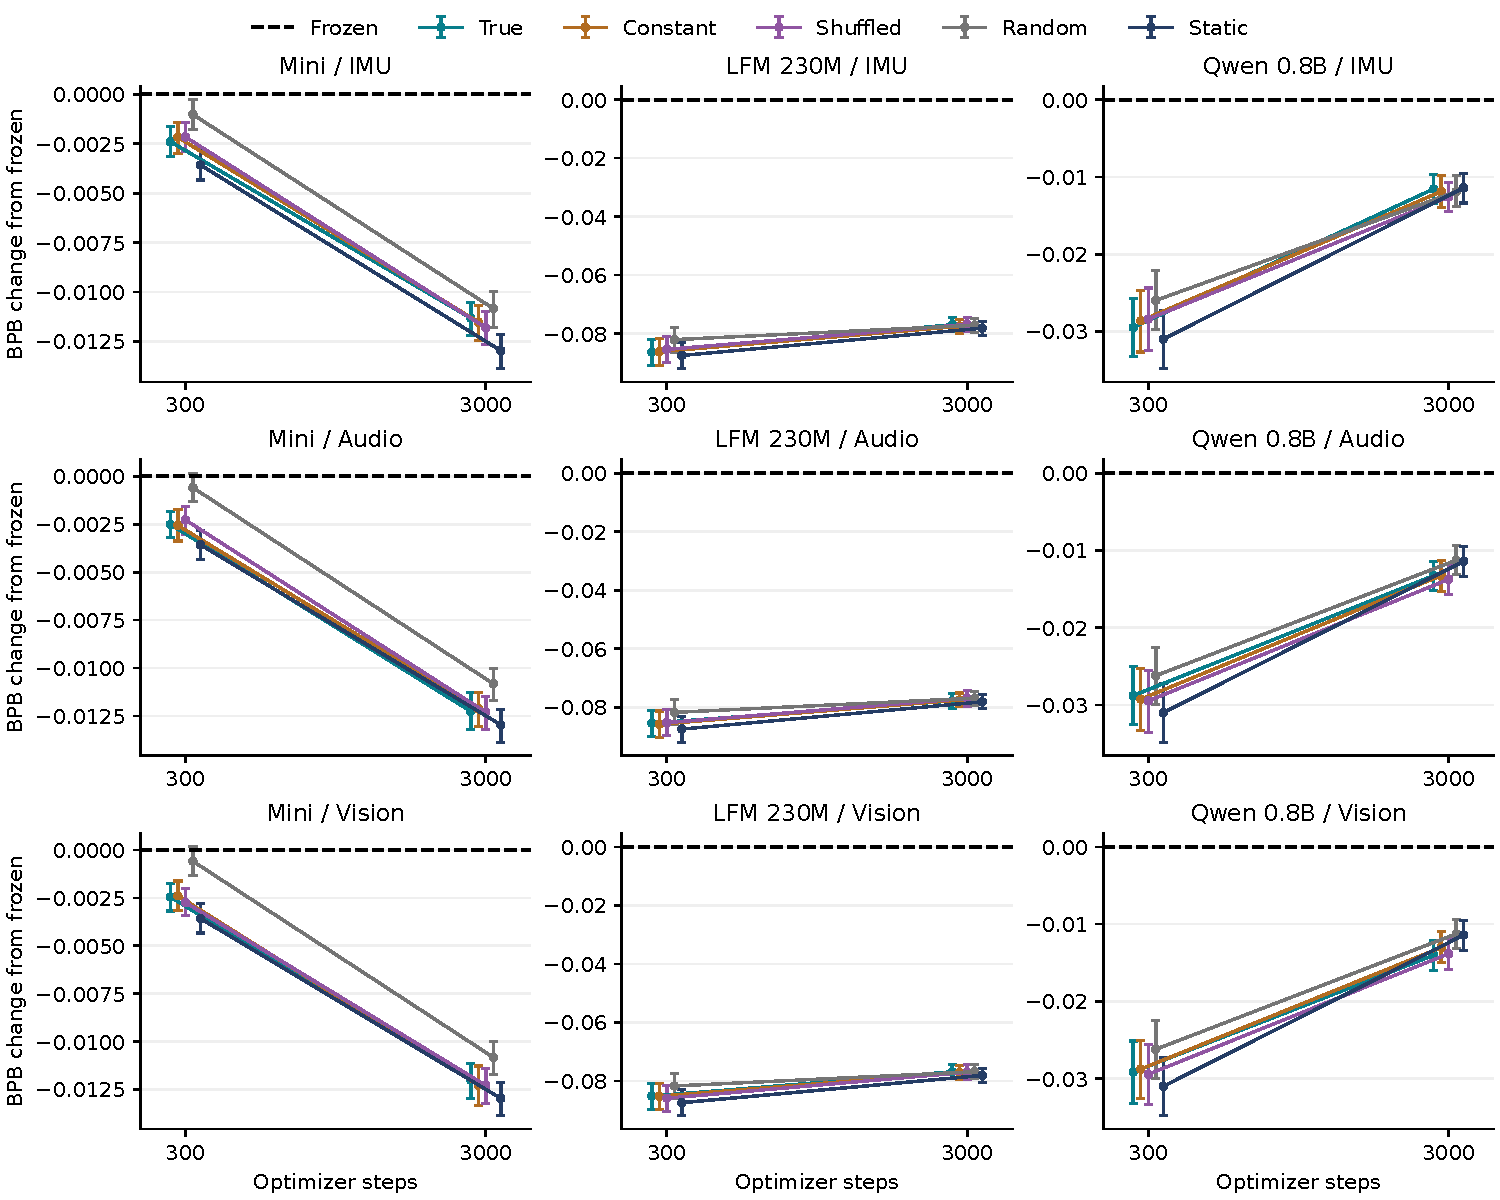
\includegraphics[width=\linewidth]{bpb-controls.pdf}
\caption{Unpaired text adaptation at the two fixed budgets. Values are paired
native-BPB differences from the frozen host on the matching evaluation panel;
negative values improve likelihood. The 300-step panel has 256 rows and the
3000-step panel has 1024, so these are within-panel changes, not identical test
samples across budgets. All plotted conditions have their registered seeds.
The common-byte table uses a separate fixed panel at both budgets.}
\label{fig:bpb}\end{figure}
\begin{table}[!htbp]\centering\small
\setlength{\tabcolsep}{4pt}
\caption{Eight generated input-prefix embeddings: native BPB at initialization and both budgets. Initialization and 300 steps use 256 rows; 3000 steps use 1024. Compare each score with the frozen reference on the same panel; the panels differ across budgets. Each score includes the same 128 text positions as its reference.}\label{tab:prefix}
\begin{tabular}{@{}lllll@{}}
\toprule
Host & Task & Initialized & 300 steps & 3000 steps \\
\midrule
Mini & IMU & 1.965 [1.928, 2.002] & 1.965 [1.928, 2.001] & 1.953 [1.934, 1.971] \\
Mini & Audio & 1.965 [1.928, 2.002] & 1.964 [1.927, 2.001] & 1.953 [1.934, 1.971] \\
Mini & Vision & 1.965 [1.929, 2.002] & 1.964 [1.927, 2.001] & 1.953 [1.934, 1.971] \\
LFM 230M & IMU & 1.192 [1.158, 1.226] & 1.114 [1.082, 1.146] & 1.070 [1.055, 1.086] \\
LFM 230M & Audio & 1.198 [1.163, 1.232] & 1.114 [1.082, 1.146] & 1.072 [1.057, 1.088] \\
LFM 230M & Vision & 1.192 [1.158, 1.225] & 1.115 [1.083, 1.147] & 1.074 [1.058, 1.090] \\
Qwen 0.8B & IMU & 1.299 [1.253, 1.344] & 1.004 [0.975, 1.033] & 0.962 [0.948, 0.976] \\
Qwen 0.8B & Audio & 1.280 [1.219, 1.347] & 1.004 [0.975, 1.033] & 0.963 [0.949, 0.977] \\
Qwen 0.8B & Vision & 1.358 [1.303, 1.414] & 1.004 [0.976, 1.033] & 0.964 [0.949, 0.978] \\
\bottomrule
\end{tabular}
\end{table}\par

At 3000 U steps, prefix-minus-frozen BPB differences range from -0.0742 to -0.0014; 9 of 9 paired intervals are below zero. Table~\ref{tab:prefix} also shows initialization and the short budget. Prefix and reference score the same 128 text positions. The result covers eight input-prefix embeddings trained on U. It does not show sensor use, and the separately trained P and G bridges provide no matched comparison of prefix conditioning.


\FloatBarrier
\subsection{Held-out sensor ranking}
Table~\ref{tab:tasks} uses all held-out items, with seed and cluster intervals. The frozen-feature linear classifier reaches macro accuracy IMU 0.967 [0.934, 0.989]; Audio 0.662 [0.624, 0.700]; Vision 0.799 [0.791, 0.807]. This reference tests whether the bridge offers value beyond information already exposed by its encoder. For the same true-trained checkpoint, the correct-minus-first-permutation macro-accuracy differences are Mini/Audio 0.443 [0.403, 0.486]; Mini/Vision 0.481 [0.426, 0.527]; LFM 230M/IMU 0.686 [0.611, 0.758]; LFM 230M/Audio 0.368 [0.317, 0.424]; Qwen 0.8B/IMU 0.685 [0.582, 0.775]; Qwen 0.8B/Audio 0.402 [0.363, 0.438]; Qwen 0.8B/Vision 0.351 [0.248, 0.455]. All five fixed permutations and other feature interventions are retained, so this first-permutation display is not selected by outcome.

The new vision probes give Mini rank-1 accuracy 0.582 [0.526, 0.628], correct-minus-different-class difference 0.536 [0.474, 0.586]; Qwen 0.8B rank-1 accuracy 0.451 [0.353, 0.553], correct-minus-different-class difference 0.389 [0.280, 0.505]. They directly test whether image features affect label ranking, addressing a question that U's BPB result cannot answer. This is a ten-class ranking test, not visual generation or open-world reasoning.

\begin{table}[!htbp]\centering\small
\setlength{\tabcolsep}{4pt}
\caption{Full-population macro rank-1 accuracy at 6000 P steps, with no diversity penalty. Uniform-choice references are 1/6 (IMU), 1/50 (audio), and 1/10 (vision). Mini/Qwen IMU/audio use five seeds; other paired cells use three. LFM vision P is outside the registered grid.}\label{tab:tasks}
\begin{tabular}{@{}llllllll@{}}
\toprule
Host & Task & Frozen & Static & Const. & Shuf. & Rand. & True [95\%] \\
\midrule
Mini & IMU & 0.167 & 0.167 & -- & -- & 0.190 & -- \\
Mini & Audio & 0.020 & 0.020 & 0.020 & 0.020 & 0.021 & 0.461 [0.419, 0.506] \\
Mini & Vision & 0.100 & 0.100 & 0.100 & -- & 0.112 & 0.582 [0.526, 0.628] \\
LFM 230M & IMU & 0.167 & 0.167 & 0.167 & 0.176 & 0.109 & 0.839 [0.761, 0.913] \\
LFM 230M & Audio & 0.020 & 0.020 & 0.018 & 0.020 & 0.023 & 0.386 [0.336, 0.442] \\
Qwen 0.8B & IMU & 0.167 & 0.167 & 0.167 & 0.173 & 0.175 & 0.838 [0.733, 0.927] \\
Qwen 0.8B & Audio & 0.020 & 0.020 & 0.021 & 0.020 & 0.023 & 0.421 [0.383, 0.459] \\
Qwen 0.8B & Vision & 0.100 & 0.100 & 0.100 & 0.100 & 0.100 & 0.451 [0.353, 0.553] \\
\bottomrule
\end{tabular}
\end{table}\par

\begin{figure}[t]\centering
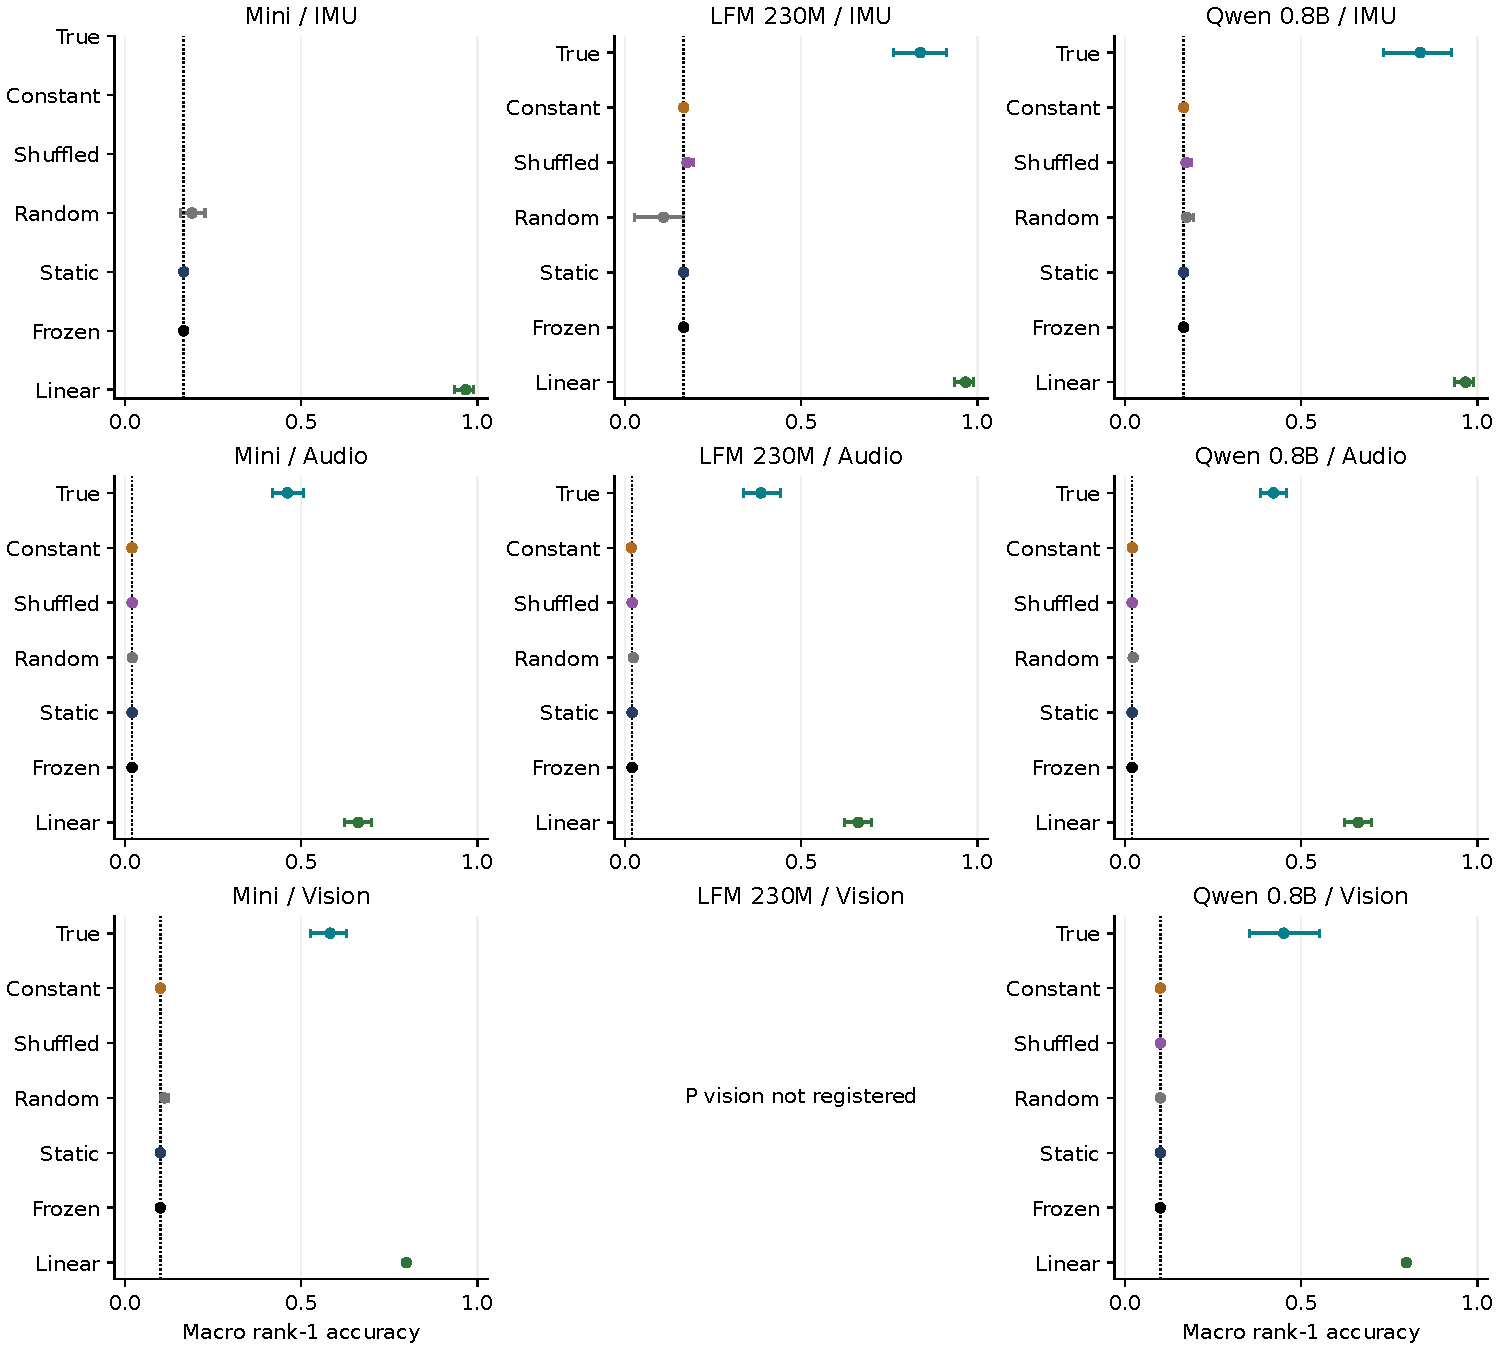
\includegraphics[width=\linewidth]{task-controls.pdf}
\caption{Macro rank-1 accuracy for the separately paired-trained P adapters at
6000 steps. The full test population and grouped intervals replace the original
64-item primary evaluation. Frozen feature classifiers measure information
already available in the encoder features.}
\label{fig:tasks}\end{figure}
\begin{table}[!htbp]\centering\small
\setlength{\tabcolsep}{4pt}
\caption{Test interventions on identical true-trained P checkpoints at 6000 steps and zero penalty. Values are macro accuracy. Different-class substitution guarantees a changed class; a permutation can retain it. Paired intervals, random features, and all five permutations are in the machine-readable analysis.}\label{tab:interventions}
\begin{tabular}{@{}lllllll@{}}
\toprule
Host & Task & Correct & Constant & Off & Other class & Shuffle 0 \\
\midrule
Mini & IMU & -- & -- & -- & -- & -- \\
Mini & Audio & 0.461 & 0.020 & 0.020 & 0.010 & 0.019 \\
Mini & Vision & 0.582 & 0.100 & 0.100 & 0.047 & 0.101 \\
LFM 230M & IMU & 0.839 & 0.167 & 0.167 & 0.032 & 0.152 \\
LFM 230M & Audio & 0.386 & 0.020 & 0.020 & 0.011 & 0.018 \\
Qwen 0.8B & IMU & 0.838 & 0.167 & 0.167 & 0.032 & 0.153 \\
Qwen 0.8B & Audio & 0.421 & 0.020 & 0.020 & 0.013 & 0.020 \\
Qwen 0.8B & Vision & 0.451 & 0.100 & 0.100 & 0.062 & 0.100 \\
\bottomrule
\end{tabular}
\end{table}\par


\FloatBarrier
\subsection{Budget, regularization, and conditioning}
Figure~\ref{fig:trajectories} connects each IMU P accuracy curve to effective-update cosine and fixed-text output sensitivity from the same weights. Table~\ref{tab:budget-endpoints} compares 600 with 6000 steps using only seeds 42, 1042, and 2042 at every penalty.

\begin{table}[!htbp]\centering\small
\setlength{\tabcolsep}{4pt}
\caption{IMU P macro rank-1 accuracy and grouped 95\% intervals for the three shared seeds. The zero-penalty row uses the same seed subset as every other penalty; additional primary probe seeds do not enter these curves. Dashes mark unavailable full-seed estimates.}\label{tab:budget-endpoints}
\begin{tabular}{@{}llll@{}}
\toprule
Host & $\lambda$ & 600 steps [95\%] & 6000 steps [95\%] \\
\midrule
Mini & 0 & 0.741 [0.693, 0.784] & -- \\
Mini & 0.01 & 0.802 [0.770, 0.830] & -- \\
Mini & 0.05 & -- & -- \\
Mini & 0.1 & 0.759 [0.701, 0.804] & -- \\
Mini & 0.2 & 0.804 [0.725, 0.903] & -- \\
LFM 230M & 0 & 0.834 [0.759, 0.911] & 0.839 [0.761, 0.913] \\
LFM 230M & 0.01 & 0.723 [0.644, 0.809] & 0.768 [0.645, 0.869] \\
LFM 230M & 0.05 & 0.759 [0.651, 0.908] & 0.741 [0.652, 0.802] \\
LFM 230M & 0.1 & 0.709 [0.623, 0.794] & 0.676 [0.640, 0.729] \\
LFM 230M & 0.2 & 0.733 [0.628, 0.820] & 0.737 [0.658, 0.840] \\
Qwen 0.8B & 0 & 0.862 [0.747, 0.956] & 0.788 [0.655, 0.911] \\
Qwen 0.8B & 0.01 & 0.738 [0.638, 0.833] & 0.607 [0.553, 0.649] \\
Qwen 0.8B & 0.05 & 0.756 [0.690, 0.821] & 0.762 [0.653, 0.867] \\
Qwen 0.8B & 0.1 & 0.667 [0.484, 0.820] & 0.762 [0.692, 0.834] \\
Qwen 0.8B & 0.2 & 0.820 [0.680, 0.923] & 0.838 [0.718, 0.929] \\
\bottomrule
\end{tabular}
\end{table}\par


Recorded numerical stops prevent complete three-seed 6000-step estimates for Mini (5 of 5 penalty settings). These gaps do not supply a later accuracy measurement. Earlier per-seed evidence remains available. At zero penalty, the 600-to-6000-step comparison is LFM 230M 0.834 [0.759, 0.911] to 0.839 [0.761, 0.913]; Qwen 0.8B 0.862 [0.747, 0.956] to 0.788 [0.655, 0.911]. The available larger-host long-endpoint intervals lie above the six-class chance rate. They do not support a universal collapse-to-chance claim at this budget.

At the largest declared penalty, $\lambda=0.2$, and 6000 P steps, the seed means are LFM 230M: factor cosine 0.145, effective-update cosine 0.694, and output KL 0.979 nats; Qwen 0.8B: factor cosine 0.009, effective-update cosine 0.790, and output KL 1.396 nats. Factor-space diversity, effective-update direction, and output variation are distinct. Cosine also does not measure update magnitude; centered energies and norms remain in the full analysis. Penalty effects differ across hosts and budgets. The full U trajectories are retained in the analysis. No penalty is selected by its test-set peak, and the short budget does not define a universal collapse threshold.

\begin{figure}[t]\centering
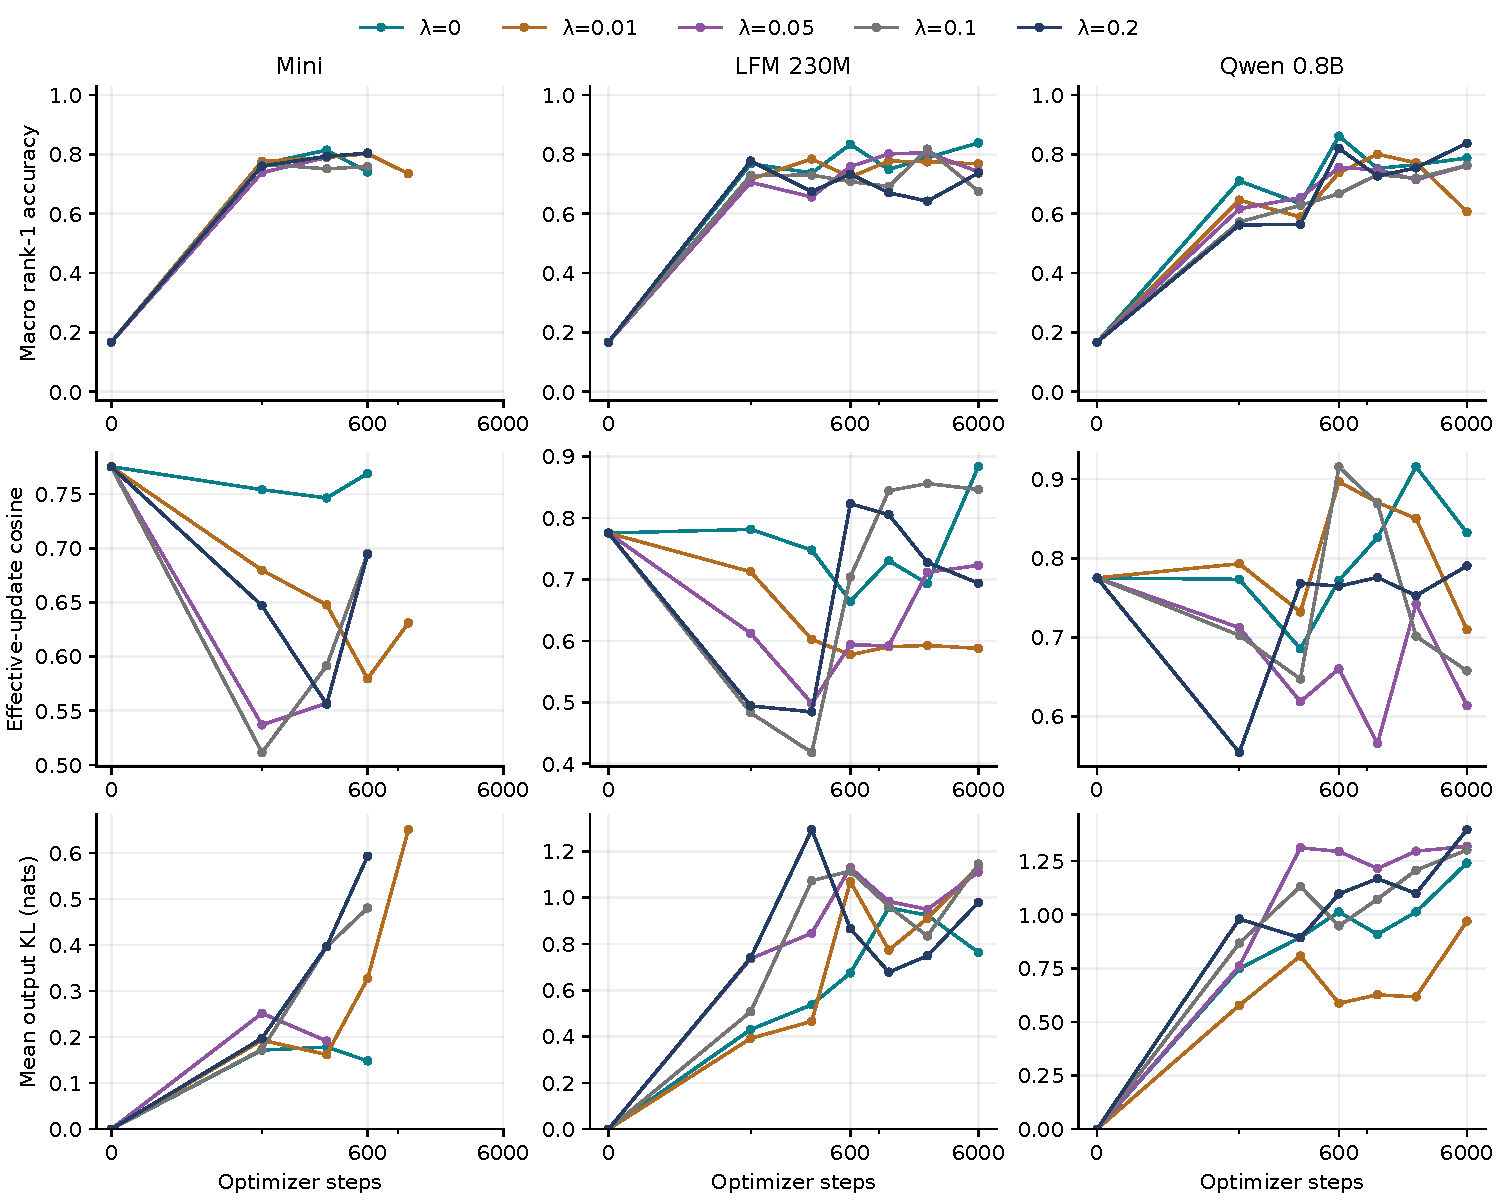
\includegraphics[width=\linewidth]{imu-trajectories.pdf}
\caption{IMU P trajectories with the registered diversity penalties. Accuracy,
effective-update geometry, and output sensitivity use the same saved weights
at each point. Intermediate checkpoints are repeated measurements of a
trajectory, not additional seeds. All penalties use three shared seeds.
Only complete three-seed estimates are drawn; curves end when numerical stops
prevent later estimates. Endpoint intervals are in Table~\ref{tab:budget-endpoints}.}
\label{fig:trajectories}\end{figure}

\FloatBarrier
\subsection{From ranking to generated responses}
Tables~\ref{tab:generation}--\ref{tab:raw-generation} distinguish raw P decoding, separately trained instruction responses, and label-in-text references. All values below are class-macro scores on held-out templates at 6000 G steps.

For IMU, label success is 0.838 [0.737, 0.936] (correct-minus-different-class 0.832 [0.731, 0.933]); sentence success is 0.689 [0.198, 0.971] (correct-minus-different-class 0.686 [0.198, 0.966]). Per-seed label scores are 0.928, 0.740, 0.847; sentence scores are 0.916, 0.193, 0.959, in seed order 42, 1042, 2042.

For Audio, label success is 0.056 [0.000, 0.161] (correct-minus-different-class 0.051 [0.000, 0.144]); sentence success is 0.064 [0.000, 0.186] (correct-minus-different-class 0.060 [0.000, 0.167]). Per-seed label scores are 0.000, 0.000, 0.169; sentence scores are 0.000, 0.000, 0.192, in seed order 42, 1042, 2042. Two of the three seeds have zero exact success in both families.

For held-out rule prompts, the differences in macro-averaged joint success (correct sensor minus a sensor from another class) are IMU $-2.1\times10^{-4}$ [-0.007, 0.004]; Audio -0.001 [-0.007, 0.006]. Requiring both reversed mappings to be correct for the same sensor and template gives the secondary scores IMU 0.005 [0.001, 0.013]; Audio 0.001 [0.000, 0.002]. Reversing the output mapping while keeping the sensor fixed tests whether responses follow the supplied rule as well as the sensor. These deterministic templates cannot demonstrate general instruction following, and sensor-dependent labels or fixed sentences alone do not show reliable rule application. The label-in-text references are practical comparisons with a different input interface; their architectures are not matched to the bridge. The evidence includes every response, including invalid and repetitive output.

\begin{table}[!htbp]\centering\small
\setlength{\tabcolsep}{4pt}
\caption{Qwen G at 6000 steps: class-macro response scores on held-out instruction templates. Each estimate requires all three training seeds. Joint success requires the exact normalized target; semantic and format scores identify different failure types.}\label{tab:generation}
\begin{tabular}{@{}lllll@{}}
\toprule
Task & Family & Semantic [95\%] & Format [95\%] & Joint [95\%] \\
\midrule
IMU & Label & 0.877 [0.748, 0.979] & 0.892 [0.799, 0.987] & 0.838 [0.737, 0.936] \\
IMU & Sentence & 0.866 [0.729, 0.971] & 0.731 [0.196, 1.000] & 0.689 [0.198, 0.971] \\
IMU & Rule & 0.501 [0.497, 0.505] & 0.999 [0.998, 1.000] & 0.501 [0.497, 0.505] \\
Audio & Label & 0.058 [0.000, 0.166] & 0.224 [0.000, 0.668] & 0.056 [0.000, 0.161] \\
Audio & Sentence & 0.064 [0.000, 0.185] & 0.281 [0.000, 0.838] & 0.064 [0.000, 0.186] \\
Audio & Rule & 0.158 [0.000, 0.468] & 0.316 [0.000, 0.937] & 0.158 [0.000, 0.468] \\
\bottomrule
\end{tabular}
\end{table}\par
\begin{table}[!htbp]\centering\small
\setlength{\tabcolsep}{4pt}
\caption{Generation references: joint success averaged by class on held-out templates, using the same G prompts and decoding. Oracle and classifier prompts give the frozen host an explicit label; other prompts supply no label text. The full analysis includes intervals and both budgets.}\label{tab:generation-controls}
\begin{tabular}{@{}lllllllll@{}}
\toprule
Task & Family & Frozen & Const. & Shuf. & Rand. & Static & Oracle & Classifier \\
\midrule
IMU & Label & 0.000 & 0.167 & 0.167 & 0.167 & 0.148 & 0.778 & 0.757 \\
IMU & Sentence & 0.000 & 0.159 & 0.139 & 0.205 & 0.130 & 0.500 & 0.484 \\
IMU & Rule & 0.162 & 0.498 & 0.460 & 0.500 & 0.446 & 0.504 & 0.502 \\
Audio & Label & 0.000 & 0.016 & 0.020 & 0.022 & 0.020 & 0.587 & 0.381 \\
Audio & Sentence & 0.000 & 0.017 & 0.013 & 0.019 & 0.020 & 0.533 & 0.347 \\
Audio & Rule & 0.226 & 0.500 & 0.500 & 0.499 & 0.500 & 0.531 & 0.465 \\
\bottomrule
\end{tabular}
\end{table}\par
\begin{table}[!htbp]\centering\small
\setlength{\tabcolsep}{4pt}
\caption{Raw generation from Qwen P checkpoints at 6000 steps, without additional instruction training. The frozen reference uses the identical original ranking prompt. Exact category output is joint success, averaged by class. This diagnostic is separate from native-chat G training.}\label{tab:raw-generation}
\begin{tabular}{@{}llll@{}}
\toprule
Task & Frozen [95\%] & P static [95\%] & P true bridge [95\%] \\
\midrule
IMU & 0.000 [0.000, 0.000] & 0.000 [0.000, 0.000] & 0.000 [0.000, 0.000] \\
Audio & 0.000 [0.000, 0.000] & 0.000 [0.000, 0.000] & 0.000 [0.000, 0.000] \\
Vision & 0.000 [0.000, 0.000] & 0.000 [0.000, 0.000] & 0.000 [0.000, 0.000] \\
\bottomrule
\end{tabular}
\end{table}\par

\FloatBarrier
{\small
\setlength{\tabcolsep}{4pt}
\begin{longtable}{@{}p{.13\linewidth}p{.37\linewidth}p{.13\linewidth}p{.28\linewidth}@{}}
\caption{Fixed examples: first registered sensor of each modality, seed 42, 6000 G steps, test template 0. The sentence and both rule mappings are shown regardless of success. Responses longer than 280 characters are visibly truncated here; the evidence retains complete output.}\label{tab:examples}\\
\toprule
Sensor & Held-out instruction & Target & Response \\
\midrule\endfirsthead
\toprule
Sensor & Held-out instruction & Target & Response \\
\midrule\endhead
IMU/\allowbreak{}uci-har/\allowbreak{}test/\allowbreak{}01155 & Complete this report with the observed category: The activity is CATEGORY. & The activity is walking. & The activity is walking. \\
IMU/\allowbreak{}uci-har/\allowbreak{}test/\allowbreak{}01155 & For this sensor reading, map category walking to yes and all remaining categories to no. Return the mapped word. & yes & yes \\
IMU/\allowbreak{}uci-har/\allowbreak{}test/\allowbreak{}01155 & For this sensor reading, map category walking to no and all remaining categories to yes. Return the mapped word. & no & yes \\
Audio/\allowbreak{}5-103415-A-2.wav & Complete this report with the observed category: The sound is CATEGORY. & The sound is pig. & !\allowbreak{}!\allowbreak{}!\allowbreak{}!\allowbreak{}!\allowbreak{}!\allowbreak{}!\allowbreak{}!\allowbreak{}!\allowbreak{}!\allowbreak{}!\allowbreak{}!\allowbreak{}!\allowbreak{}!\allowbreak{}!\allowbreak{}!\allowbreak{}!\allowbreak{}!\allowbreak{}!\allowbreak{}!\allowbreak{}!\allowbreak{}!\allowbreak{}!\allowbreak{}!\allowbreak{}!\allowbreak{}!\allowbreak{}!\allowbreak{}!\allowbreak{}!\allowbreak{}!\allowbreak{}!\allowbreak{}!\allowbreak{}!\allowbreak{}!\allowbreak{}!\allowbreak{}!\allowbreak{}!\allowbreak{}!\allowbreak{}!\allowbreak{}!\allowbreak{}!\allowbreak{}!\allowbreak{}!\allowbreak{}!\allowbreak{}!\allowbreak{}!\allowbreak{}!\allowbreak{}!\allowbreak{}!\allowbreak{}!\allowbreak{}!\allowbreak{}!\allowbreak{}!\allowbreak{}!\allowbreak{}!\allowbreak{}!\allowbreak{}!\allowbreak{}!\allowbreak{}!\allowbreak{}!\allowbreak{}!\allowbreak{}!\allowbreak{}!\allowbreak{}!\allowbreak{} \\
Audio/\allowbreak{}5-103415-A-2.wav & For this sensor reading, map category pig to yes and all remaining categories to no. Return the mapped word. & yes & !\allowbreak{}!\allowbreak{}!\allowbreak{}!\allowbreak{}!\allowbreak{}!\allowbreak{}!\allowbreak{}!\allowbreak{}!\allowbreak{}!\allowbreak{}!\allowbreak{}!\allowbreak{}!\allowbreak{}!\allowbreak{}!\allowbreak{}!\allowbreak{}!\allowbreak{}!\allowbreak{}!\allowbreak{}!\allowbreak{}!\allowbreak{}!\allowbreak{}!\allowbreak{}!\allowbreak{}!\allowbreak{}!\allowbreak{}!\allowbreak{}!\allowbreak{}!\allowbreak{}!\allowbreak{}!\allowbreak{}!\allowbreak{}!\allowbreak{}!\allowbreak{}!\allowbreak{}!\allowbreak{}!\allowbreak{}!\allowbreak{}!\allowbreak{}!\allowbreak{}!\allowbreak{}!\allowbreak{}!\allowbreak{}!\allowbreak{}!\allowbreak{}!\allowbreak{}!\allowbreak{}!\allowbreak{}!\allowbreak{}!\allowbreak{}!\allowbreak{}!\allowbreak{}!\allowbreak{}!\allowbreak{}!\allowbreak{}!\allowbreak{}!\allowbreak{}!\allowbreak{}!\allowbreak{}!\allowbreak{}!\allowbreak{}!\allowbreak{}!\allowbreak{}!\allowbreak{} \\
Audio/\allowbreak{}5-103415-A-2.wav & For this sensor reading, map category pig to no and all remaining categories to yes. Return the mapped word. & no & !\allowbreak{}!\allowbreak{}!\allowbreak{}!\allowbreak{}!\allowbreak{}!\allowbreak{}!\allowbreak{}!\allowbreak{}!\allowbreak{}!\allowbreak{}!\allowbreak{}!\allowbreak{}!\allowbreak{}!\allowbreak{}!\allowbreak{}!\allowbreak{}!\allowbreak{}!\allowbreak{}!\allowbreak{}!\allowbreak{}!\allowbreak{}!\allowbreak{}!\allowbreak{}!\allowbreak{}!\allowbreak{}!\allowbreak{}!\allowbreak{}!\allowbreak{}!\allowbreak{}!\allowbreak{}!\allowbreak{}!\allowbreak{}!\allowbreak{}!\allowbreak{}!\allowbreak{}!\allowbreak{}!\allowbreak{}!\allowbreak{}!\allowbreak{}!\allowbreak{}!\allowbreak{}!\allowbreak{}!\allowbreak{}!\allowbreak{}!\allowbreak{}!\allowbreak{}!\allowbreak{}!\allowbreak{}!\allowbreak{}!\allowbreak{}!\allowbreak{}!\allowbreak{}!\allowbreak{}!\allowbreak{}!\allowbreak{}!\allowbreak{}!\allowbreak{}!\allowbreak{}!\allowbreak{}!\allowbreak{}!\allowbreak{}!\allowbreak{}!\allowbreak{}!\allowbreak{} \\
\bottomrule
\end{longtable}}\par


A separate fixed-batch diagnostic explains the repeated exclamation marks in
two G/audio seeds. On the first forward pass, finite but very large activations
overflow the FP32 mean square in the final RMS normalization, which returns
zeros. At every decoding step the logits are all zero; the greedy tie rule
selects token zero, \texttt{!}, through the token limit. The third seed has no
normalization overflow in this inspected batch. The hooks preserve the
registered arithmetic and reproduce the saved responses. These observations
cover only the first eight cases for one audio clip; they establish a numerical
cause for those outputs, not its incidence across the generation panel or the
effect of changing normalization arithmetic. This output degeneration should
not be interpreted as evidence of finite, input-independent conditioning
collapse. The public package supplies the observations and a
\texttt{diagnose-generation} command.


\FloatBarrier
\subsection{Composition and resource cost}
\label{sec:cost}
For matched U constituents at 150 or 1500 steps, we test all seven modality
subsets. Historical factor averaging computes
$(\sum_j A_j/k)(\sum_j B_j/k)$, which includes cross terms. Effective-update sum
computes $\sum_j A_jB_j$; effective mean divides that sum by $k$. These are
different operators. We evaluate them with identical constituent checkpoints,
text rows, and per-modality feature cycles, without rank recompression. The
streams remain unpaired, so this is an adapter-interference test, not evidence
of semantic multi-sensor reasoning.
\begin{table}[!htbp]\centering\small
\setlength{\tabcolsep}{4pt}
\caption{All three U modalities composed at 1500 constituent steps. Negative changes from frozen improve BPB. Positive nonadditivity means combined BPB is worse than the prediction from summing standalone BPB improvements. We use that prediction as a descriptive reference. The analysis includes all subsets and both budgets.}\label{tab:composition}
\begin{tabular}{@{}lllll@{}}
\toprule
Host & Operator & BPB [95\%] & $\Delta$ frozen [95\%] & Nonadditivity [95\%] \\
\midrule
Mini & Update mean & 1.945 [1.927, 1.963] & -0.009 [-0.010, -0.009] & 0.010 [0.009, 0.011] \\
Mini & Update sum & 2.000 [1.981, 2.018] & 0.046 [0.043, 0.048] & 0.065 [0.063, 0.066] \\
Mini & Factor mean & 1.949 [1.931, 1.967] & -0.005 [-0.005, -0.005] & 0.014 [0.013, 0.016] \\
LFM 230M & Update mean & 1.059 [1.044, 1.075] & -0.085 [-0.088, -0.083] & 0.145 [0.141, 0.150] \\
LFM 230M & Update sum & 1.193 [1.177, 1.210] & 0.049 [0.044, 0.053] & 0.279 [0.273, 0.286] \\
LFM 230M & Factor mean & 1.070 [1.055, 1.086] & -0.074 [-0.077, -0.072] & 0.156 [0.151, 0.162] \\
Qwen 0.8B & Update mean & 0.965 [0.951, 0.979] & -0.033 [-0.035, -0.031] & 0.009 [0.005, 0.013] \\
Qwen 0.8B & Update sum & 1.103 [1.088, 1.118] & 0.105 [0.100, 0.110] & 0.147 [0.142, 0.152] \\
Qwen 0.8B & Factor mean & 0.966 [0.951, 0.980] & -0.032 [-0.034, -0.031] & 0.010 [0.005, 0.014] \\
\bottomrule
\end{tabular}
\end{table}\par


Table~\ref{tab:resources} reports measured costs, including the frozen encoder. Across successfully trained trajectories, training records contain Mini 5.24 accumulated optimizer-step hours and 1.94 GiB peak allocated training memory; LFM 230M 12.20 accumulated optimizer-step hours and 5.04 GiB peak allocated training memory; Qwen 0.8B 76.44 accumulated optimizer-step hours and 17.58 GiB peak allocated training memory. These step times include batch preparation and synchronized training, but exclude model loading, checkpoint writes, separate evaluation, and failed attempts. The artifact also records the wall time of each successful worker attempt. Times overlap under concurrent training and are not isolated GPU-hours or total elapsed study time. The measurements include dense-head cost rather than inferring efficiency from the number of adapted host parameters.

\begin{table}[!htbp]\centering\small
\setlength{\tabcolsep}{4pt}
\caption{Resource measurements at batch size one on the isolated RTX PRO 6000. Parameters are millions of trainable adapter parameters. VRAM is peak allocated GiB with the host, adapter, and external encoder resident. First is median time from raw sensor input to the first token, in milliseconds; 32-token is median generation time with cached sensor factors and a fresh text cache. Both use 128 input text tokens. Frozen/static paths skip unused sensor work. The appendix contains every modality and prefix case.}\label{tab:resources}
\begin{tabular}{@{}lllllll@{}}
\toprule
Host & Task & Interface & Params M & VRAM GiB & First ms & 32-token ms \\
\midrule
Mini & IMU & Bridge & 84.33 & 0.49 & 3.7 & 90.0 \\
Mini & IMU & None & 0.00 & 0.17 & 1.8 & 49.8 \\
Mini & IMU & Static & 0.33 & 0.17 & 2.7 & 82.3 \\
LFM 230M & IMU & Bridge & 199.07 & 1.67 & 6.5 & 161.0 \\
LFM 230M & IMU & None & 0.00 & 0.93 & 4.2 & 113.4 \\
LFM 230M & IMU & Static & 0.77 & 0.93 & 5.7 & 158.6 \\
Qwen 0.8B & IMU & Bridge & 410.66 & 4.52 & 50.6 & 440.1 \\
Qwen 0.8B & IMU & None & 0.00 & 2.99 & 46.8 & 359.8 \\
Qwen 0.8B & IMU & Static & 1.60 & 2.99 & 49.4 & 423.0 \\
\bottomrule
\end{tabular}
\end{table}\par

Batch-one timings use one isolated RTX PRO 6000, 128 input text tokens, and
32 generated tokens. Raw inputs are already decoded in memory. The artifact
separates preprocessing, encoding, adapter generation, prefill, and generation,
and distinguishes a fresh sensor from cached factors. It records the device
power limit, temperature, and clocks around each case. Native LFM/Qwen decoding
uses a new text cache for each request; the released mini implementation
recomputes its prefix. Repeat dispersion measures variability in this setup,
not uncertainty across devices or applications. No edge-device efficiency
claim follows from these workstation measurements.

\section{Related work}
Hypernetworks generate the parameters of another network~\cite{ha2016hypernetworks}.
Adapters~\cite{houlsby2019adapters}, LoRA~\cite{hu2021lora}, shared
hypernetwork adapters~\cite{mahabadi2021hyperformer}, and
HyperTuning~\cite{phang2022hypertuning} motivate adapting frozen hosts through
smaller trainable interfaces. The bridge studied here conditions generated
LoRA factors on continuous external encoder features. Its dense output head
is substantial, so ``frozen host'' and ``parameter efficient'' are separate
properties. Prompt tuning becomes more competitive with scale in the T5
experiments of Lester et al.~\cite{lester2021power}; our fixed input-prefix
comparison is narrower in architecture and optimization.

The earlier 230M companion note (Paper 2 in this series) used the historical
protocol~\cite{penov2026bridges230m}. This revision supplies new LFM comparisons
with corrected evaluation and seed coverage; the companion's artifacts remain
separate. The compression study (Paper 3) replaces the dense output head with
coefficients over a learned or frozen basis of LoRA
directions~\cite{penov2026compressed}. We retain the dense head here to measure
its cost and behavior under the shared recipe. The compression study's results
describe its separate architecture and protocol.

Multimodal systems such as Flamingo~\cite{alayrac2022flamingo} and
LLaVA~\cite{liu2023llava} study broader visual-language behavior with different
interfaces and supervision. Our closed-set ranking and deterministic response
tasks do not establish comparable capability. Weight-space composition is
related to task arithmetic~\cite{ilharco2023task}, but separately generated
low-rank factors require care: factor averaging is not addition of their
effective updates.

\section{Limitations and interpretation}
The bridge can be modular while remaining expensive. It still requires paired
examples for P and G and does not eliminate supervision for a new sensor task.
The external encoders already expose strong label information; a linear
classifier and label-in-text baseline are essential practical comparisons.
Label ranking and short generated responses establish bounded behavior, not
open-ended descriptions, compositional cross-modal reasoning, or robust
real-world sensor use.

The larger-host comparison remains below one billion nominal language-model
parameters and changes several host properties together. One shared optimizer
recipe is useful for a controlled replication but cannot establish each
interface's best achievable performance. Unpaired-text results should not be
generalized to paired likelihood objectives. Prefix observations should not be
generalized to all soft prompts or per-layer prefixes. Geometric diversity
should not be equated with correct conditioning.

Audio normalization exposure and incomplete original encoder provenance limit
the strength of end-to-end holdout claims. The source-disjoint sensitivity
analysis addresses a narrower overlap only. Fixed test subjects, one audio
holdout fold, image-domain transfer, and unknown host pretraining exposure
further bound generalization. We retain negative outcomes and all declared
budgets; the study does not choose a checkpoint or penalty from test accuracy.

\section{Reproducibility and revision record}
The public reproduction package is
\url{https://github.com/kortexa-ai/legolm.paper/tree/main/paper1}.
All papers remain on the main branch with explicit per-paper entry points.
The package has its own namespace and dependency lock. It includes the exact
mini tokenizer, pinned input identities, all recipes, checkpoint hashes,
per-item evaluation evidence, and an artifact-only verification command.
Model execution and artifact verification are separate documented workflows.
The verified summary drives the primary empirical tables, figures, and result
text. The separate fixed-batch normalization observations are supplied in
\href{https://github.com/kortexa-ai/legolm.paper/blob/main/paper1/artifacts/revision-2/diagnostics/g-audio-normalization.json}{the generation diagnostic artifact}. Exact FP32 adapter checkpoints have a separate
download index with immutable URLs, sizes, and hashes. The same index supplies
the exact frozen feature caches, so encoder arithmetic on another device need
not change a checkpoint's input features. Checkpoints can be evaluated without
repeating training. Regenerating them from scratch requires the
documented input assets and compute.

A revision audit found that the initial native-chat decoder inherited only
the model EOS and continued past valid assistant endings. A saved-checkpoint
replay reproduced repeated answers. We corrected the stopping rule and
rescored the saved checkpoints. Source-version reconciliation excludes the
earlier decoding results from reported scores.

The original root-level \texttt{arxiv/} and \texttt{src/} remain the historical release. This revision replaces its primary estimates with the corrected, explicitly registered matrix. Changes include matched prefix text budgets, separation of training and test corruption, native tokenization at label boundaries, full-population evaluation, and fresh larger-host runs. The new results must not be pooled with historical scores from a different evaluation protocol. The matrix identifier is \texttt{1942c97abc73}. The evidence manifest SHA-256 is recorded in \texttt{release.json}, along with the exact summary and rendering sources. The source archive includes its bibliography and is compiled in a fresh directory before release. The original mini tokenizer is distributed exactly; it is not reconstructed from a new tokenizer-training run.


\bibliographystyle{plain}
\bibliography{references}
\clearpage
\appendix
\section{Complete registered comparisons}
The machine-readable summary contains every condition, seed estimate, paired contrast, intervention, and intermediate checkpoint. The following tables retain both primary endpoints and the declared penalty values. A final release accounts for every declared trial, including numerical failures. For an unavailable aggregate, $n=a/b$ gives available/declared seeds; no survivor-only estimate is reported.

{\small
\setlength{\tabcolsep}{4pt}
\begin{longtable}{@{}lllllll@{}}
\caption{Numerical failures under the fixed recipe. A range is bounded by the original execution log; the separate diagnostic replay is not a replacement trial. Saved checkpoints before failure remain in the evidence.}\label{tab:numerical-failures}\\
\toprule
Host/cohort & Task & Interface & Seed & $\lambda$ & Failure step & Unavailable steps \\
\midrule\endfirsthead
\toprule
Host/cohort & Task & Interface & Seed & $\lambda$ & Failure step & Unavailable steps \\
\midrule\endhead
Mini/P & IMU & bridge/constant & 1042 & 0 & 2853 & 6000 \\
Mini/P & IMU & bridge/constant & 2042 & 0 & 5088 & 6000 \\
Mini/P & IMU & bridge/constant & 3042 & 0 & 3031 & 6000 \\
Mini/P & IMU & bridge/constant & 42 & 0 & 5009 & 6000 \\
Mini/P & IMU & bridge/shuffled & 1042 & 0 & 3295 & 6000 \\
Mini/P & IMU & bridge/shuffled & 2042 & 0 & 2520 & 6000 \\
Mini/P & IMU & bridge/shuffled & 42 & 0 & 3211 & 6000 \\
Mini/P & Vision & bridge/shuffled & 42 & 0 & 4347 & 6000 \\
Mini/P & IMU & bridge/true & 1042 & 0 & 1263 & 2400, 6000 \\
Mini/P & IMU & bridge/true & 2042 & 0 & 1170 & 1200, 2400, 6000 \\
Mini/P & IMU & bridge/true & 3042 & 0 & 1069 & 1200, 2400, 6000 \\
Mini/P & IMU & bridge/true & 4042 & 0 & 1823 & 2400, 6000 \\
Mini/P & IMU & bridge/true & 42 & 0 & 1301--1350 & 2400, 6000 \\
Mini/P & IMU & bridge/true & 1042 & 0.01 & 2211 & 2400, 6000 \\
Mini/P & IMU & bridge/true & 2042 & 0.01 & 2143 & 2400, 6000 \\
Mini/P & IMU & bridge/true & 42 & 0.01 & 2580 & 6000 \\
Mini/P & IMU & bridge/true & 1042 & 0.05 & 1388 & 2400, 6000 \\
Mini/P & IMU & bridge/true & 2042 & 0.05 & 5112 & 6000 \\
Mini/P & IMU & bridge/true & 42 & 0.05 & 545 & 600, 1200, 2400, 6000 \\
Mini/P & IMU & bridge/true & 1042 & 0.1 & 889 & 1200, 2400, 6000 \\
Mini/P & IMU & bridge/true & 2042 & 0.1 & 4007 & 6000 \\
Mini/P & IMU & bridge/true & 42 & 0.1 & 1698 & 2400, 6000 \\
Mini/P & IMU & bridge/true & 1042 & 0.2 & 807 & 1200, 2400, 6000 \\
Mini/P & IMU & bridge/true & 2042 & 0.2 & 2936 & 6000 \\
Mini/P & IMU & bridge/true & 42 & 0.2 & 1118 & 1200, 2400, 6000 \\
\bottomrule
\end{longtable}}\par

{\small
\setlength{\tabcolsep}{4pt}
\begin{longtable}{@{}llllllll@{}}
\caption{Native BPB; step/row count is shown explicitly. $n$ is the number of training seeds; a frozen host is a fixed reference.}\label{tab:full-native_bpb}\\
\toprule
Host & Task & Interface & $\lambda$ & Step/rows & $n$ & BPB [95\%] & Seed SD \\
\midrule\endfirsthead
\toprule
Host & Task & Interface & $\lambda$ & Step/rows & $n$ & BPB [95\%] & Seed SD \\
\midrule\endhead
LFM 230M & Audio & constant & 0 & 3000/1024 & 3 & 1.067 [1.052, 1.083] & $1.2\times10^{-4}$ \\
LFM 230M & Audio & constant & 0 & 300/256 & 3 & 1.098 [1.066, 1.131] & 0.001 \\
LFM 230M & IMU & constant & 0 & 3000/1024 & 3 & 1.067 [1.052, 1.083] & 0.001 \\
LFM 230M & IMU & constant & 0 & 300/256 & 3 & 1.098 [1.065, 1.130] & 0.001 \\
LFM 230M & Vision & constant & 0 & 3000/1024 & 3 & 1.067 [1.052, 1.083] & $4.3\times10^{-4}$ \\
LFM 230M & Vision & constant & 0 & 300/256 & 3 & 1.099 [1.066, 1.131] & 0.002 \\
Mini & Audio & constant & 0 & 3000/1024 & 3 & 1.942 [1.924, 1.960] & $2.5\times10^{-4}$ \\
Mini & Audio & constant & 0 & 300/256 & 3 & 1.963 [1.926, 1.999] & $4.3\times10^{-4}$ \\
Mini & IMU & constant & 0 & 3000/1024 & 3 & 1.943 [1.925, 1.961] & $3.3\times10^{-4}$ \\
Mini & IMU & constant & 0 & 300/256 & 3 & 1.963 [1.926, 2.000] & $3.3\times10^{-4}$ \\
Mini & Vision & constant & 0 & 3000/1024 & 3 & 1.942 [1.924, 1.960] & 0.001 \\
Mini & Vision & constant & 0 & 300/256 & 3 & 1.963 [1.926, 2.000] & $3.3\times10^{-4}$ \\
Qwen 0.8B & Audio & constant & 0 & 3000/1024 & 3 & 0.985 [0.970, 0.999] & 0.001 \\
Qwen 0.8B & Audio & constant & 0 & 300/256 & 3 & 1.010 [0.981, 1.039] & 0.001 \\
Qwen 0.8B & IMU & constant & 0 & 3000/1024 & 3 & 0.986 [0.972, 1.000] & 0.001 \\
Qwen 0.8B & IMU & constant & 0 & 300/256 & 3 & 1.011 [0.982, 1.040] & 0.001 \\
Qwen 0.8B & Vision & constant & 0 & 3000/1024 & 3 & 0.985 [0.971, 0.999] & 0.001 \\
Qwen 0.8B & Vision & constant & 0 & 300/256 & 3 & 1.011 [0.982, 1.039] & 0.001 \\
LFM 230M & Audio & random & 0 & 3000/1024 & 3 & 1.068 [1.052, 1.084] & $4.1\times10^{-4}$ \\
LFM 230M & Audio & random & 0 & 300/256 & 3 & 1.102 [1.070, 1.135] & $4.7\times10^{-4}$ \\
LFM 230M & IMU & random & 0 & 3000/1024 & 3 & 1.067 [1.052, 1.083] & $3.4\times10^{-4}$ \\
LFM 230M & IMU & random & 0 & 300/256 & 3 & 1.102 [1.070, 1.134] & 0.001 \\
LFM 230M & Vision & random & 0 & 3000/1024 & 3 & 1.068 [1.052, 1.084] & $4.1\times10^{-4}$ \\
LFM 230M & Vision & random & 0 & 300/256 & 3 & 1.102 [1.070, 1.135] & $4.7\times10^{-4}$ \\
Mini & Audio & random & 0 & 3000/1024 & 3 & 1.943 [1.925, 1.961] & $2.6\times10^{-4}$ \\
Mini & Audio & random & 0 & 300/256 & 3 & 1.965 [1.928, 2.001] & $2.5\times10^{-4}$ \\
Mini & IMU & random & 0 & 3000/1024 & 3 & 1.943 [1.925, 1.961] & $4.8\times10^{-4}$ \\
Mini & IMU & random & 0 & 300/256 & 3 & 1.964 [1.927, 2.001] & $3.3\times10^{-4}$ \\
Mini & Vision & random & 0 & 3000/1024 & 3 & 1.943 [1.925, 1.961] & $2.6\times10^{-4}$ \\
Mini & Vision & random & 0 & 300/256 & 3 & 1.965 [1.928, 2.001] & $2.5\times10^{-4}$ \\
Qwen 0.8B & Audio & random & 0 & 3000/1024 & 3 & 0.987 [0.973, 1.001] & $8.9\times10^{-5}$ \\
Qwen 0.8B & Audio & random & 0 & 300/256 & 3 & 1.013 [0.984, 1.042] & 0.001 \\
Qwen 0.8B & IMU & random & 0 & 3000/1024 & 3 & 0.986 [0.972, 1.000] & 0.001 \\
Qwen 0.8B & IMU & random & 0 & 300/256 & 3 & 1.014 [0.985, 1.042] & 0.002 \\
Qwen 0.8B & Vision & random & 0 & 3000/1024 & 3 & 0.987 [0.973, 1.001] & $8.9\times10^{-5}$ \\
Qwen 0.8B & Vision & random & 0 & 300/256 & 3 & 1.013 [0.984, 1.042] & 0.001 \\
LFM 230M & Audio & shuffled & 0 & 3000/1024 & 3 & 1.068 [1.052, 1.084] & 0.001 \\
LFM 230M & Audio & shuffled & 0 & 300/256 & 3 & 1.099 [1.066, 1.131] & 0.001 \\
LFM 230M & IMU & shuffled & 0 & 3000/1024 & 3 & 1.068 [1.052, 1.084] & $3.6\times10^{-4}$ \\
LFM 230M & IMU & shuffled & 0 & 300/256 & 3 & 1.099 [1.066, 1.131] & 0.001 \\
LFM 230M & Vision & shuffled & 0 & 3000/1024 & 3 & 1.068 [1.052, 1.084] & 0.001 \\
LFM 230M & Vision & shuffled & 0 & 300/256 & 3 & 1.098 [1.066, 1.130] & $4.5\times10^{-4}$ \\
Mini & Audio & shuffled & 0 & 3000/1024 & 3 & 1.942 [1.924, 1.960] & $1.3\times10^{-4}$ \\
Mini & Audio & shuffled & 0 & 300/256 & 3 & 1.963 [1.926, 2.000] & $2.1\times10^{-4}$ \\
Mini & IMU & shuffled & 0 & 3000/1024 & 3 & 1.942 [1.924, 1.960] & $2.3\times10^{-4}$ \\
Mini & IMU & shuffled & 0 & 300/256 & 3 & 1.963 [1.926, 2.000] & $1.3\times10^{-4}$ \\
Mini & Vision & shuffled & 0 & 3000/1024 & 3 & 1.942 [1.924, 1.960] & $3.5\times10^{-4}$ \\
Mini & Vision & shuffled & 0 & 300/256 & 3 & 1.963 [1.926, 1.999] & $2.2\times10^{-4}$ \\
Qwen 0.8B & Audio & shuffled & 0 & 3000/1024 & 3 & 0.984 [0.970, 0.999] & $2.7\times10^{-4}$ \\
Qwen 0.8B & Audio & shuffled & 0 & 300/256 & 3 & 1.010 [0.981, 1.039] & 0.002 \\
Qwen 0.8B & IMU & shuffled & 0 & 3000/1024 & 3 & 0.985 [0.971, 1.000] & $4.6\times10^{-4}$ \\
Qwen 0.8B & IMU & shuffled & 0 & 300/256 & 3 & 1.011 [0.982, 1.040] & 0.002 \\
Qwen 0.8B & Vision & shuffled & 0 & 3000/1024 & 3 & 0.984 [0.970, 0.998] & 0.001 \\
Qwen 0.8B & Vision & shuffled & 0 & 300/256 & 3 & 1.010 [0.981, 1.039] & 0.001 \\
LFM 230M & Audio & true & 0 & 3000/1024 & 3 & 1.067 [1.051, 1.083] & 0.001 \\
LFM 230M & Audio & true & 0 & 300/256 & 3 & 1.098 [1.066, 1.131] & $4.0\times10^{-4}$ \\
LFM 230M & IMU & true & 0 & 3000/1024 & 3 & 1.068 [1.052, 1.084] & $1.6\times10^{-4}$ \\
LFM 230M & IMU & true & 0 & 300/256 & 3 & 1.098 [1.065, 1.130] & 0.001 \\
LFM 230M & Vision & true & 0 & 3000/1024 & 3 & 1.068 [1.052, 1.084] & $3.1\times10^{-4}$ \\
LFM 230M & Vision & true & 0 & 300/256 & 3 & 1.099 [1.066, 1.131] & $4.9\times10^{-4}$ \\
LFM 230M & Audio & Frozen & 0 & 0/1024 & 1 & 1.145 [1.128, 1.161] & -- \\
LFM 230M & Audio & Frozen & 0 & 0/256 & 1 & 1.184 [1.150, 1.218] & -- \\
LFM 230M & IMU & Frozen & 0 & 0/1024 & 1 & 1.145 [1.128, 1.161] & -- \\
LFM 230M & IMU & Frozen & 0 & 0/256 & 1 & 1.184 [1.150, 1.218] & -- \\
LFM 230M & Vision & Frozen & 0 & 0/1024 & 1 & 1.145 [1.128, 1.161] & -- \\
LFM 230M & Vision & Frozen & 0 & 0/256 & 1 & 1.184 [1.150, 1.218] & -- \\
LFM 230M & Audio & prefix & 0 & 3000/1024 & 3 & 1.072 [1.057, 1.088] & $1.1\times10^{-4}$ \\
LFM 230M & Audio & prefix & 0 & 0/256 & 3 & 1.198 [1.163, 1.232] & 0.003 \\
LFM 230M & Audio & prefix & 0 & 300/256 & 3 & 1.114 [1.082, 1.146] & 0.001 \\
LFM 230M & IMU & prefix & 0 & 3000/1024 & 3 & 1.070 [1.055, 1.086] & $1.3\times10^{-4}$ \\
LFM 230M & IMU & prefix & 0 & 0/256 & 3 & 1.192 [1.158, 1.226] & 0.005 \\
LFM 230M & IMU & prefix & 0 & 300/256 & 3 & 1.114 [1.082, 1.146] & 0.001 \\
LFM 230M & Vision & prefix & 0 & 3000/1024 & 3 & 1.074 [1.058, 1.090] & $4.7\times10^{-4}$ \\
LFM 230M & Vision & prefix & 0 & 0/256 & 3 & 1.192 [1.158, 1.225] & 0.001 \\
LFM 230M & Vision & prefix & 0 & 300/256 & 3 & 1.115 [1.083, 1.147] & $3.9\times10^{-4}$ \\
LFM 230M & Audio & static & 0 & 3000/1024 & 3 & 1.066 [1.051, 1.083] & $1.4\times10^{-4}$ \\
LFM 230M & Audio & static & 0 & 300/256 & 3 & 1.096 [1.064, 1.129] & $9.9\times10^{-5}$ \\
LFM 230M & IMU & static & 0 & 3000/1024 & 3 & 1.066 [1.051, 1.083] & $1.4\times10^{-4}$ \\
LFM 230M & IMU & static & 0 & 300/256 & 3 & 1.096 [1.064, 1.129] & $9.9\times10^{-5}$ \\
LFM 230M & Vision & static & 0 & 3000/1024 & 3 & 1.066 [1.051, 1.083] & $1.4\times10^{-4}$ \\
LFM 230M & Vision & static & 0 & 300/256 & 3 & 1.096 [1.064, 1.129] & $9.9\times10^{-5}$ \\
Mini & Audio & true & 0 & 3000/1024 & 3 & 1.942 [1.924, 1.960] & 0.001 \\
Mini & Audio & true & 0 & 300/256 & 3 & 1.963 [1.926, 1.999] & $1.9\times10^{-4}$ \\
Mini & IMU & true & 0 & 3000/1024 & 3 & 1.943 [1.925, 1.961] & $1.7\times10^{-4}$ \\
Mini & IMU & true & 0 & 300/256 & 3 & 1.963 [1.926, 1.999] & $3.4\times10^{-4}$ \\
Mini & Vision & true & 0 & 3000/1024 & 3 & 1.942 [1.924, 1.960] & $3.1\times10^{-4}$ \\
Mini & Vision & true & 0 & 300/256 & 3 & 1.963 [1.926, 1.999] & $7.9\times10^{-5}$ \\
Mini & Audio & Frozen & 0 & 0/1024 & 1 & 1.954 [1.936, 1.973] & -- \\
Mini & Audio & Frozen & 0 & 0/256 & 1 & 1.965 [1.929, 2.004] & -- \\
Mini & IMU & Frozen & 0 & 0/1024 & 1 & 1.954 [1.936, 1.973] & -- \\
Mini & IMU & Frozen & 0 & 0/256 & 1 & 1.965 [1.929, 2.004] & -- \\
Mini & Vision & Frozen & 0 & 0/1024 & 1 & 1.954 [1.936, 1.973] & -- \\
Mini & Vision & Frozen & 0 & 0/256 & 1 & 1.965 [1.929, 2.004] & -- \\
Mini & Audio & prefix & 0 & 3000/1024 & 3 & 1.953 [1.934, 1.971] & $4.8\times10^{-5}$ \\
Mini & Audio & prefix & 0 & 0/256 & 3 & 1.965 [1.928, 2.002] & $1.5\times10^{-4}$ \\
Mini & Audio & prefix & 0 & 300/256 & 3 & 1.964 [1.927, 2.001] & $6.7\times10^{-5}$ \\
Mini & IMU & prefix & 0 & 3000/1024 & 3 & 1.953 [1.934, 1.971] & $3.5\times10^{-5}$ \\
Mini & IMU & prefix & 0 & 0/256 & 3 & 1.965 [1.928, 2.002] & $2.0\times10^{-4}$ \\
Mini & IMU & prefix & 0 & 300/256 & 3 & 1.965 [1.928, 2.001] & $2.6\times10^{-4}$ \\
Mini & Vision & prefix & 0 & 3000/1024 & 3 & 1.953 [1.934, 1.971] & $2.9\times10^{-5}$ \\
Mini & Vision & prefix & 0 & 0/256 & 3 & 1.965 [1.929, 2.002] & $8.4\times10^{-5}$ \\
Mini & Vision & prefix & 0 & 300/256 & 3 & 1.964 [1.927, 2.001] & $4.4\times10^{-6}$ \\
Mini & Audio & static & 0 & 3000/1024 & 3 & 1.941 [1.923, 1.959] & $1.4\times10^{-4}$ \\
Mini & Audio & static & 0 & 300/256 & 3 & 1.962 [1.925, 1.998] & $1.5\times10^{-4}$ \\
Mini & IMU & static & 0 & 3000/1024 & 3 & 1.941 [1.923, 1.959] & $1.4\times10^{-4}$ \\
Mini & IMU & static & 0 & 300/256 & 3 & 1.962 [1.925, 1.998] & $1.5\times10^{-4}$ \\
Mini & Vision & static & 0 & 3000/1024 & 3 & 1.941 [1.923, 1.959] & $1.4\times10^{-4}$ \\
Mini & Vision & static & 0 & 300/256 & 3 & 1.962 [1.925, 1.998] & $1.5\times10^{-4}$ \\
Qwen 0.8B & Audio & true & 0 & 3000/1024 & 3 & 0.985 [0.971, 0.999] & $1.7\times10^{-4}$ \\
Qwen 0.8B & Audio & true & 0 & 300/256 & 3 & 1.011 [0.982, 1.040] & 0.001 \\
Qwen 0.8B & IMU & true & 0 & 3000/1024 & 3 & 0.986 [0.972, 1.001] & $3.5\times10^{-4}$ \\
Qwen 0.8B & IMU & true & 0 & 300/256 & 3 & 1.010 [0.981, 1.039] & 0.001 \\
Qwen 0.8B & Vision & true & 0 & 3000/1024 & 3 & 0.984 [0.970, 0.998] & 0.001 \\
Qwen 0.8B & Vision & true & 0 & 300/256 & 3 & 1.010 [0.981, 1.039] & 0.001 \\
Qwen 0.8B & Audio & Frozen & 0 & 0/1024 & 1 & 0.998 [0.984, 1.012] & -- \\
Qwen 0.8B & Audio & Frozen & 0 & 0/256 & 1 & 1.040 [1.010, 1.069] & -- \\
Qwen 0.8B & IMU & Frozen & 0 & 0/1024 & 1 & 0.998 [0.984, 1.012] & -- \\
Qwen 0.8B & IMU & Frozen & 0 & 0/256 & 1 & 1.040 [1.010, 1.069] & -- \\
Qwen 0.8B & Vision & Frozen & 0 & 0/1024 & 1 & 0.998 [0.984, 1.012] & -- \\
Qwen 0.8B & Vision & Frozen & 0 & 0/256 & 1 & 1.040 [1.010, 1.069] & -- \\
Qwen 0.8B & Audio & prefix & 0 & 3000/1024 & 3 & 0.963 [0.949, 0.977] & $4.1\times10^{-4}$ \\
Qwen 0.8B & Audio & prefix & 0 & 0/256 & 3 & 1.280 [1.219, 1.347] & 0.058 \\
Qwen 0.8B & Audio & prefix & 0 & 300/256 & 3 & 1.004 [0.975, 1.033] & $2.5\times10^{-4}$ \\
Qwen 0.8B & IMU & prefix & 0 & 3000/1024 & 3 & 0.962 [0.948, 0.976] & $2.7\times10^{-4}$ \\
Qwen 0.8B & IMU & prefix & 0 & 0/256 & 3 & 1.299 [1.253, 1.344] & 0.026 \\
Qwen 0.8B & IMU & prefix & 0 & 300/256 & 3 & 1.004 [0.975, 1.033] & 0.001 \\
Qwen 0.8B & Vision & prefix & 0 & 3000/1024 & 3 & 0.964 [0.949, 0.978] & 0.001 \\
Qwen 0.8B & Vision & prefix & 0 & 0/256 & 3 & 1.358 [1.303, 1.414] & 0.043 \\
Qwen 0.8B & Vision & prefix & 0 & 300/256 & 3 & 1.004 [0.976, 1.033] & 0.001 \\
Qwen 0.8B & Audio & static & 0 & 3000/1024 & 3 & 0.987 [0.972, 1.001] & 0.001 \\
Qwen 0.8B & Audio & static & 0 & 300/256 & 3 & 1.009 [0.979, 1.037] & $2.3\times10^{-4}$ \\
Qwen 0.8B & IMU & static & 0 & 3000/1024 & 3 & 0.987 [0.972, 1.001] & 0.001 \\
Qwen 0.8B & IMU & static & 0 & 300/256 & 3 & 1.009 [0.979, 1.037] & $2.3\times10^{-4}$ \\
Qwen 0.8B & Vision & static & 0 & 3000/1024 & 3 & 0.987 [0.972, 1.001] & 0.001 \\
Qwen 0.8B & Vision & static & 0 & 300/256 & 3 & 1.009 [0.979, 1.037] & $2.3\times10^{-4}$ \\
LFM 230M & IMU & true & 0.01 & 3000/1024 & 3 & 1.068 [1.052, 1.084] & $3.4\times10^{-4}$ \\
LFM 230M & IMU & true & 0.01 & 300/256 & 3 & 1.099 [1.067, 1.131] & 0.001 \\
Mini & IMU & true & 0.01 & 3000/1024 & 3 & 1.943 [1.925, 1.961] & $3.5\times10^{-4}$ \\
Mini & IMU & true & 0.01 & 300/256 & 3 & 1.963 [1.926, 2.000] & $3.6\times10^{-4}$ \\
Qwen 0.8B & IMU & true & 0.01 & 3000/1024 & 3 & 0.985 [0.971, 0.999] & $3.8\times10^{-4}$ \\
Qwen 0.8B & IMU & true & 0.01 & 300/256 & 3 & 1.010 [0.980, 1.039] & 0.002 \\
LFM 230M & IMU & true & 0.05 & 3000/1024 & 3 & 1.068 [1.052, 1.084] & $2.1\times10^{-4}$ \\
LFM 230M & IMU & true & 0.05 & 300/256 & 3 & 1.099 [1.067, 1.131] & $3.6\times10^{-4}$ \\
Mini & IMU & true & 0.05 & 3000/1024 & 3 & 1.949 [1.931, 1.967] & $4.9\times10^{-4}$ \\
Mini & IMU & true & 0.05 & 300/256 & 3 & 1.965 [1.928, 2.001] & 0.001 \\
Qwen 0.8B & IMU & true & 0.05 & 3000/1024 & 3 & 0.985 [0.971, 0.999] & 0.001 \\
Qwen 0.8B & IMU & true & 0.05 & 300/256 & 3 & 1.010 [0.981, 1.039] & 0.002 \\
LFM 230M & IMU & true & 0.1 & 3000/1024 & 3 & 1.068 [1.053, 1.084] & 0.001 \\
LFM 230M & IMU & true & 0.1 & 300/256 & 3 & 1.106 [1.074, 1.138] & 0.002 \\
Mini & IMU & true & 0.1 & 3000/1024 & 3 & 1.949 [1.931, 1.968] & $2.2\times10^{-4}$ \\
Mini & IMU & true & 0.1 & 300/256 & 3 & 1.965 [1.928, 2.002] & 0.001 \\
Qwen 0.8B & IMU & true & 0.1 & 3000/1024 & 3 & 0.986 [0.972, 1.000] & $2.4\times10^{-4}$ \\
Qwen 0.8B & IMU & true & 0.1 & 300/256 & 3 & 1.009 [0.979, 1.037] & 0.001 \\
LFM 230M & IMU & true & 0.2 & 3000/1024 & 3 & 1.072 [1.057, 1.088] & $3.3\times10^{-4}$ \\
LFM 230M & IMU & true & 0.2 & 300/256 & 3 & 1.111 [1.078, 1.143] & 0.001 \\
Mini & IMU & true & 0.2 & 3000/1024 & 3 & 1.949 [1.931, 1.967] & 0.001 \\
Mini & IMU & true & 0.2 & 300/256 & 3 & 1.966 [1.929, 2.002] & 0.001 \\
Qwen 0.8B & IMU & true & 0.2 & 3000/1024 & 3 & 0.988 [0.974, 1.002] & 0.001 \\
Qwen 0.8B & IMU & true & 0.2 & 300/256 & 3 & 1.017 [0.988, 1.047] & 0.002 \\
\bottomrule
\end{longtable}}\par

{\small
\setlength{\tabcolsep}{4pt}
\begin{longtable}{@{}llllllll@{}}
\caption{Common-byte BPB on identical held-out spans. $n$ is the number of training seeds; a frozen host is a fixed reference.}\label{tab:full-common_bpb}\\
\toprule
Host & Task & Interface & $\lambda$ & Step & $n$ & BPB [95\%] & Seed SD \\
\midrule\endfirsthead
\toprule
Host & Task & Interface & $\lambda$ & Step & $n$ & BPB [95\%] & Seed SD \\
\midrule\endhead
LFM 230M & Audio & constant & 0 & 3000 & 3 & 1.268 [1.237, 1.300] & 0.001 \\
LFM 230M & Audio & constant & 0 & 300 & 3 & 1.271 [1.240, 1.302] & 0.001 \\
LFM 230M & IMU & constant & 0 & 3000 & 3 & 1.268 [1.238, 1.300] & 0.001 \\
LFM 230M & IMU & constant & 0 & 300 & 3 & 1.272 [1.241, 1.304] & 0.002 \\
LFM 230M & Vision & constant & 0 & 3000 & 3 & 1.270 [1.239, 1.301] & $4.3\times10^{-4}$ \\
LFM 230M & Vision & constant & 0 & 300 & 3 & 1.271 [1.240, 1.302] & 0.002 \\
Mini & Audio & constant & 0 & 3000 & 3 & 2.122 [2.082, 2.164] & $3.6\times10^{-4}$ \\
Mini & Audio & constant & 0 & 300 & 3 & 2.139 [2.098, 2.182] & $2.8\times10^{-4}$ \\
Mini & IMU & constant & 0 & 3000 & 3 & 2.124 [2.083, 2.165] & $4.2\times10^{-4}$ \\
Mini & IMU & constant & 0 & 300 & 3 & 2.140 [2.099, 2.182] & $2.5\times10^{-4}$ \\
Mini & Vision & constant & 0 & 3000 & 3 & 2.122 [2.081, 2.164] & $1.6\times10^{-4}$ \\
Mini & Vision & constant & 0 & 300 & 3 & 2.139 [2.098, 2.181] & $4.8\times10^{-4}$ \\
Qwen 0.8B & Audio & constant & 0 & 3000 & 3 & 1.189 [1.161, 1.217] & $3.7\times10^{-4}$ \\
Qwen 0.8B & Audio & constant & 0 & 300 & 3 & 1.179 [1.151, 1.206] & 0.001 \\
Qwen 0.8B & IMU & constant & 0 & 3000 & 3 & 1.187 [1.160, 1.216] & 0.001 \\
Qwen 0.8B & IMU & constant & 0 & 300 & 3 & 1.183 [1.155, 1.210] & 0.002 \\
Qwen 0.8B & Vision & constant & 0 & 3000 & 3 & 1.187 [1.159, 1.216] & 0.001 \\
Qwen 0.8B & Vision & constant & 0 & 300 & 3 & 1.180 [1.153, 1.207] & 0.001 \\
LFM 230M & Audio & random & 0 & 3000 & 3 & 1.270 [1.239, 1.301] & $4.1\times10^{-4}$ \\
LFM 230M & Audio & random & 0 & 300 & 3 & 1.276 [1.245, 1.307] & 0.001 \\
LFM 230M & IMU & random & 0 & 3000 & 3 & 1.269 [1.238, 1.301] & 0.002 \\
LFM 230M & IMU & random & 0 & 300 & 3 & 1.276 [1.245, 1.307] & $4.6\times10^{-4}$ \\
LFM 230M & Vision & random & 0 & 3000 & 3 & 1.270 [1.239, 1.301] & $4.1\times10^{-4}$ \\
LFM 230M & Vision & random & 0 & 300 & 3 & 1.276 [1.245, 1.307] & 0.001 \\
Mini & Audio & random & 0 & 3000 & 3 & 2.125 [2.084, 2.166] & $9.0\times10^{-5}$ \\
Mini & Audio & random & 0 & 300 & 3 & 2.141 [2.101, 2.184] & 0.001 \\
Mini & IMU & random & 0 & 3000 & 3 & 2.125 [2.084, 2.166] & $3.3\times10^{-4}$ \\
Mini & IMU & random & 0 & 300 & 3 & 2.141 [2.100, 2.183] & 0.001 \\
Mini & Vision & random & 0 & 3000 & 3 & 2.125 [2.084, 2.166] & $9.0\times10^{-5}$ \\
Mini & Vision & random & 0 & 300 & 3 & 2.141 [2.101, 2.184] & 0.001 \\
Qwen 0.8B & Audio & random & 0 & 3000 & 3 & 1.190 [1.162, 1.219] & 0.002 \\
Qwen 0.8B & Audio & random & 0 & 300 & 3 & 1.182 [1.155, 1.210] & 0.001 \\
Qwen 0.8B & IMU & random & 0 & 3000 & 3 & 1.189 [1.161, 1.217] & 0.003 \\
Qwen 0.8B & IMU & random & 0 & 300 & 3 & 1.184 [1.156, 1.212] & 0.001 \\
Qwen 0.8B & Vision & random & 0 & 3000 & 3 & 1.190 [1.162, 1.219] & 0.002 \\
Qwen 0.8B & Vision & random & 0 & 300 & 3 & 1.182 [1.155, 1.210] & 0.001 \\
LFM 230M & Audio & shuffled & 0 & 3000 & 3 & 1.269 [1.238, 1.300] & 0.002 \\
LFM 230M & Audio & shuffled & 0 & 300 & 3 & 1.272 [1.240, 1.303] & $4.4\times10^{-4}$ \\
LFM 230M & IMU & shuffled & 0 & 3000 & 3 & 1.270 [1.239, 1.301] & 0.001 \\
LFM 230M & IMU & shuffled & 0 & 300 & 3 & 1.271 [1.240, 1.302] & 0.001 \\
LFM 230M & Vision & shuffled & 0 & 3000 & 3 & 1.268 [1.237, 1.299] & 0.002 \\
LFM 230M & Vision & shuffled & 0 & 300 & 3 & 1.270 [1.239, 1.301] & $4.5\times10^{-4}$ \\
Mini & Audio & shuffled & 0 & 3000 & 3 & 2.122 [2.082, 2.164] & 0.001 \\
Mini & Audio & shuffled & 0 & 300 & 3 & 2.140 [2.099, 2.182] & 0.001 \\
Mini & IMU & shuffled & 0 & 3000 & 3 & 2.124 [2.083, 2.165] & $3.7\times10^{-4}$ \\
Mini & IMU & shuffled & 0 & 300 & 3 & 2.139 [2.098, 2.181] & $1.7\times10^{-4}$ \\
Mini & Vision & shuffled & 0 & 3000 & 3 & 2.122 [2.082, 2.164] & 0.001 \\
Mini & Vision & shuffled & 0 & 300 & 3 & 2.139 [2.098, 2.181] & $2.4\times10^{-4}$ \\
Qwen 0.8B & Audio & shuffled & 0 & 3000 & 3 & 1.187 [1.159, 1.216] & 0.002 \\
Qwen 0.8B & Audio & shuffled & 0 & 300 & 3 & 1.181 [1.153, 1.209] & 0.004 \\
Qwen 0.8B & IMU & shuffled & 0 & 3000 & 3 & 1.187 [1.159, 1.216] & 0.002 \\
Qwen 0.8B & IMU & shuffled & 0 & 300 & 3 & 1.181 [1.154, 1.209] & 0.001 \\
Qwen 0.8B & Vision & shuffled & 0 & 3000 & 3 & 1.187 [1.159, 1.215] & 0.001 \\
Qwen 0.8B & Vision & shuffled & 0 & 300 & 3 & 1.180 [1.153, 1.208] & 0.001 \\
LFM 230M & Audio & true & 0 & 3000 & 3 & 1.266 [1.235, 1.298] & 0.001 \\
LFM 230M & Audio & true & 0 & 300 & 3 & 1.271 [1.240, 1.302] & $3.4\times10^{-4}$ \\
LFM 230M & IMU & true & 0 & 3000 & 3 & 1.269 [1.238, 1.300] & 0.002 \\
LFM 230M & IMU & true & 0 & 300 & 3 & 1.272 [1.241, 1.303] & 0.001 \\
LFM 230M & Vision & true & 0 & 3000 & 3 & 1.269 [1.238, 1.300] & $2.6\times10^{-4}$ \\
LFM 230M & Vision & true & 0 & 300 & 3 & 1.271 [1.240, 1.302] & 0.002 \\
LFM 230M & Audio & Frozen & 0 & 0 & 1 & 1.373 [1.340, 1.407] & -- \\
LFM 230M & IMU & Frozen & 0 & 0 & 1 & 1.373 [1.340, 1.407] & -- \\
LFM 230M & Vision & Frozen & 0 & 0 & 1 & 1.373 [1.340, 1.407] & -- \\
LFM 230M & Audio & prefix & 0 & 0 & 3 & 1.385 [1.351, 1.419] & 0.002 \\
LFM 230M & Audio & prefix & 0 & 3000 & 3 & 1.275 [1.243, 1.306] & $4.9\times10^{-4}$ \\
LFM 230M & Audio & prefix & 0 & 300 & 3 & 1.280 [1.248, 1.312] & 0.001 \\
LFM 230M & IMU & prefix & 0 & 0 & 3 & 1.382 [1.348, 1.416] & 0.001 \\
LFM 230M & IMU & prefix & 0 & 3000 & 3 & 1.274 [1.242, 1.305] & $2.8\times10^{-4}$ \\
LFM 230M & IMU & prefix & 0 & 300 & 3 & 1.282 [1.250, 1.314] & $3.5\times10^{-4}$ \\
LFM 230M & Vision & prefix & 0 & 0 & 3 & 1.379 [1.345, 1.413] & 0.004 \\
LFM 230M & Vision & prefix & 0 & 3000 & 3 & 1.276 [1.245, 1.308] & 0.001 \\
LFM 230M & Vision & prefix & 0 & 300 & 3 & 1.282 [1.251, 1.315] & 0.002 \\
LFM 230M & Audio & static & 0 & 3000 & 3 & 1.268 [1.237, 1.299] & 0.001 \\
LFM 230M & Audio & static & 0 & 300 & 3 & 1.271 [1.240, 1.303] & $2.9\times10^{-4}$ \\
LFM 230M & IMU & static & 0 & 3000 & 3 & 1.268 [1.237, 1.299] & 0.001 \\
LFM 230M & IMU & static & 0 & 300 & 3 & 1.271 [1.240, 1.303] & $2.9\times10^{-4}$ \\
LFM 230M & Vision & static & 0 & 3000 & 3 & 1.268 [1.237, 1.299] & 0.001 \\
LFM 230M & Vision & static & 0 & 300 & 3 & 1.271 [1.240, 1.303] & $2.9\times10^{-4}$ \\
Mini & Audio & true & 0 & 3000 & 3 & 2.122 [2.082, 2.164] & 0.001 \\
Mini & Audio & true & 0 & 300 & 3 & 2.139 [2.098, 2.182] & $3.3\times10^{-4}$ \\
Mini & IMU & true & 0 & 3000 & 3 & 2.123 [2.083, 2.165] & 0.001 \\
Mini & IMU & true & 0 & 300 & 3 & 2.139 [2.098, 2.181] & $4.1\times10^{-4}$ \\
Mini & Vision & true & 0 & 3000 & 3 & 2.123 [2.082, 2.165] & $4.9\times10^{-4}$ \\
Mini & Vision & true & 0 & 300 & 3 & 2.139 [2.098, 2.181] & $2.2\times10^{-4}$ \\
Mini & Audio & Frozen & 0 & 0 & 1 & 2.142 [2.103, 2.185] & -- \\
Mini & IMU & Frozen & 0 & 0 & 1 & 2.142 [2.103, 2.185] & -- \\
Mini & Vision & Frozen & 0 & 0 & 1 & 2.142 [2.103, 2.185] & -- \\
Mini & Audio & prefix & 0 & 0 & 3 & 2.144 [2.103, 2.186] & 0.001 \\
Mini & Audio & prefix & 0 & 3000 & 3 & 2.140 [2.099, 2.183] & $5.3\times10^{-5}$ \\
Mini & Audio & prefix & 0 & 300 & 3 & 2.141 [2.100, 2.184] & $3.1\times10^{-4}$ \\
Mini & IMU & prefix & 0 & 0 & 3 & 2.144 [2.103, 2.186] & $3.3\times10^{-4}$ \\
Mini & IMU & prefix & 0 & 3000 & 3 & 2.140 [2.099, 2.182] & $7.5\times10^{-5}$ \\
Mini & IMU & prefix & 0 & 300 & 3 & 2.142 [2.100, 2.184] & $4.0\times10^{-4}$ \\
Mini & Vision & prefix & 0 & 0 & 3 & 2.144 [2.103, 2.186] & 0.001 \\
Mini & Vision & prefix & 0 & 3000 & 3 & 2.140 [2.099, 2.183] & $6.7\times10^{-5}$ \\
Mini & Vision & prefix & 0 & 300 & 3 & 2.142 [2.100, 2.184] & $1.7\times10^{-4}$ \\
Mini & Audio & static & 0 & 3000 & 3 & 2.122 [2.081, 2.164] & $3.3\times10^{-4}$ \\
Mini & Audio & static & 0 & 300 & 3 & 2.138 [2.097, 2.180] & $2.0\times10^{-4}$ \\
Mini & IMU & static & 0 & 3000 & 3 & 2.122 [2.081, 2.164] & $3.3\times10^{-4}$ \\
Mini & IMU & static & 0 & 300 & 3 & 2.138 [2.097, 2.180] & $2.0\times10^{-4}$ \\
Mini & Vision & static & 0 & 3000 & 3 & 2.122 [2.081, 2.164] & $3.3\times10^{-4}$ \\
Mini & Vision & static & 0 & 300 & 3 & 2.138 [2.097, 2.180] & $2.0\times10^{-4}$ \\
Qwen 0.8B & Audio & true & 0 & 3000 & 3 & 1.187 [1.159, 1.216] & 0.001 \\
Qwen 0.8B & Audio & true & 0 & 300 & 3 & 1.180 [1.152, 1.207] & 0.002 \\
Qwen 0.8B & IMU & true & 0 & 3000 & 3 & 1.189 [1.161, 1.218] & 0.003 \\
Qwen 0.8B & IMU & true & 0 & 300 & 3 & 1.180 [1.152, 1.207] & 0.001 \\
Qwen 0.8B & Vision & true & 0 & 3000 & 3 & 1.187 [1.159, 1.215] & 0.002 \\
Qwen 0.8B & Vision & true & 0 & 300 & 3 & 1.180 [1.152, 1.208] & 0.002 \\
Qwen 0.8B & Audio & Frozen & 0 & 0 & 1 & 1.212 [1.184, 1.241] & -- \\
Qwen 0.8B & IMU & Frozen & 0 & 0 & 1 & 1.212 [1.184, 1.241] & -- \\
Qwen 0.8B & Vision & Frozen & 0 & 0 & 1 & 1.212 [1.184, 1.241] & -- \\
Qwen 0.8B & Audio & prefix & 0 & 0 & 3 & 1.611 [1.535, 1.702] & 0.084 \\
Qwen 0.8B & Audio & prefix & 0 & 3000 & 3 & 1.165 [1.137, 1.193] & 0.001 \\
Qwen 0.8B & Audio & prefix & 0 & 300 & 3 & 1.173 [1.145, 1.201] & 0.002 \\
Qwen 0.8B & IMU & prefix & 0 & 0 & 3 & 1.653 [1.577, 1.732] & 0.076 \\
Qwen 0.8B & IMU & prefix & 0 & 3000 & 3 & 1.163 [1.136, 1.191] & $2.6\times10^{-4}$ \\
Qwen 0.8B & IMU & prefix & 0 & 300 & 3 & 1.172 [1.144, 1.200] & 0.001 \\
Qwen 0.8B & Vision & prefix & 0 & 0 & 3 & 1.743 [1.671, 1.819] & 0.067 \\
Qwen 0.8B & Vision & prefix & 0 & 3000 & 3 & 1.166 [1.139, 1.194] & 0.001 \\
Qwen 0.8B & Vision & prefix & 0 & 300 & 3 & 1.173 [1.145, 1.201] & 0.001 \\
Qwen 0.8B & Audio & static & 0 & 3000 & 3 & 1.189 [1.162, 1.218] & 0.001 \\
Qwen 0.8B & Audio & static & 0 & 300 & 3 & 1.178 [1.151, 1.205] & 0.001 \\
Qwen 0.8B & IMU & static & 0 & 3000 & 3 & 1.189 [1.162, 1.218] & 0.001 \\
Qwen 0.8B & IMU & static & 0 & 300 & 3 & 1.178 [1.151, 1.205] & 0.001 \\
Qwen 0.8B & Vision & static & 0 & 3000 & 3 & 1.189 [1.162, 1.218] & 0.001 \\
Qwen 0.8B & Vision & static & 0 & 300 & 3 & 1.178 [1.151, 1.205] & 0.001 \\
LFM 230M & IMU & true & 0.01 & 3000 & 3 & 1.270 [1.239, 1.301] & 0.001 \\
LFM 230M & IMU & true & 0.01 & 300 & 3 & 1.272 [1.241, 1.304] & 0.001 \\
Mini & IMU & true & 0.01 & 3000 & 3 & 2.124 [2.084, 2.166] & 0.001 \\
Mini & IMU & true & 0.01 & 300 & 3 & 2.140 [2.098, 2.182] & $3.4\times10^{-4}$ \\
Qwen 0.8B & IMU & true & 0.01 & 3000 & 3 & 1.188 [1.160, 1.217] & 0.001 \\
Qwen 0.8B & IMU & true & 0.01 & 300 & 3 & 1.180 [1.152, 1.207] & 0.001 \\
LFM 230M & IMU & true & 0.05 & 3000 & 3 & 1.269 [1.238, 1.301] & 0.002 \\
LFM 230M & IMU & true & 0.05 & 300 & 3 & 1.272 [1.241, 1.303] & 0.001 \\
Mini & IMU & true & 0.05 & 3000 & 3 & 2.133 [2.092, 2.175] & 0.001 \\
Mini & IMU & true & 0.05 & 300 & 3 & 2.142 [2.101, 2.184] & 0.001 \\
Qwen 0.8B & IMU & true & 0.05 & 3000 & 3 & 1.188 [1.160, 1.217] & 0.001 \\
Qwen 0.8B & IMU & true & 0.05 & 300 & 3 & 1.180 [1.153, 1.208] & 0.002 \\
LFM 230M & IMU & true & 0.1 & 3000 & 3 & 1.269 [1.238, 1.301] & 0.003 \\
LFM 230M & IMU & true & 0.1 & 300 & 3 & 1.280 [1.249, 1.311] & 0.003 \\
Mini & IMU & true & 0.1 & 3000 & 3 & 2.134 [2.093, 2.176] & 0.001 \\
Mini & IMU & true & 0.1 & 300 & 3 & 2.142 [2.101, 2.184] & $1.9\times10^{-4}$ \\
Qwen 0.8B & IMU & true & 0.1 & 3000 & 3 & 1.191 [1.163, 1.219] & 0.001 \\
Qwen 0.8B & IMU & true & 0.1 & 300 & 3 & 1.177 [1.150, 1.205] & 0.002 \\
LFM 230M & IMU & true & 0.2 & 3000 & 3 & 1.276 [1.245, 1.307] & 0.001 \\
LFM 230M & IMU & true & 0.2 & 300 & 3 & 1.284 [1.253, 1.316] & 0.001 \\
Mini & IMU & true & 0.2 & 3000 & 3 & 2.132 [2.092, 2.175] & 0.001 \\
Mini & IMU & true & 0.2 & 300 & 3 & 2.143 [2.102, 2.185] & 0.001 \\
Qwen 0.8B & IMU & true & 0.2 & 3000 & 3 & 1.191 [1.163, 1.220] & 0.004 \\
Qwen 0.8B & IMU & true & 0.2 & 300 & 3 & 1.188 [1.160, 1.216] & 0.004 \\
\bottomrule
\end{longtable}}\par

{\small
\setlength{\tabcolsep}{4pt}
\begin{longtable}{@{}llllllll@{}}
\caption{Paired P ranking on the full held-out population. $n$ is the number of training seeds; a frozen host is a fixed reference.}\label{tab:full-ranking}\\
\toprule
Host & Task & Interface & $\lambda$ & Step & $n$ & Macro [95\%] & Micro [95\%] \\
\midrule\endfirsthead
\toprule
Host & Task & Interface & $\lambda$ & Step & $n$ & Macro [95\%] & Micro [95\%] \\
\midrule\endhead
LFM 230M & Audio & constant & 0 & 6000 & 3 & 0.018 [0.010, 0.022] & 0.018 [0.010, 0.024] \\
LFM 230M & Audio & constant & 0 & 600 & 3 & 0.018 [0.013, 0.022] & 0.018 [0.013, 0.024] \\
LFM 230M & IMU & constant & 0 & 6000 & 3 & 0.167 [0.167, 0.167] & 0.148 [0.138, 0.159] \\
LFM 230M & IMU & constant & 0 & 600 & 3 & 0.167 [0.167, 0.167] & 0.160 [0.155, 0.164] \\
Mini & Audio & constant & 0 & 6000 & 5 & 0.020 [0.017, 0.020] & 0.020 [0.017, 0.023] \\
Mini & Audio & constant & 0 & 600 & 5 & 0.024 [0.020, 0.029] & 0.024 [0.019, 0.029] \\
Mini & IMU & constant & 0 & 6000 & 1/5 & -- & -- \\
Mini & IMU & constant & 0 & 600 & 5 & 0.167 [0.167, 0.167] & 0.156 [0.148, 0.163] \\
Mini & Vision & constant & 0 & 6000 & 3 & 0.100 [0.100, 0.101] & 0.100 [0.100, 0.101] \\
Mini & Vision & constant & 0 & 600 & 3 & 0.100 [0.100, 0.100] & 0.100 [0.100, 0.100] \\
Qwen 0.8B & Audio & constant & 0 & 6000 & 5 & 0.021 [0.018, 0.024] & 0.021 [0.016, 0.026] \\
Qwen 0.8B & Audio & constant & 0 & 600 & 5 & 0.017 [0.011, 0.022] & 0.017 [0.010, 0.024] \\
Qwen 0.8B & IMU & constant & 0 & 6000 & 5 & 0.167 [0.167, 0.167] & 0.153 [0.144, 0.161] \\
Qwen 0.8B & IMU & constant & 0 & 600 & 5 & 0.167 [0.166, 0.167] & 0.153 [0.144, 0.161] \\
Qwen 0.8B & Vision & constant & 0 & 6000 & 3 & 0.100 [0.100, 0.100] & 0.100 [0.100, 0.100] \\
Qwen 0.8B & Vision & constant & 0 & 600 & 3 & 0.105 [0.100, 0.114] & 0.105 [0.100, 0.114] \\
LFM 230M & Audio & random & 0 & 6000 & 3 & 0.023 [0.020, 0.028] & 0.023 [0.017, 0.030] \\
LFM 230M & Audio & random & 0 & 600 & 3 & 0.024 [0.018, 0.031] & 0.024 [0.017, 0.032] \\
LFM 230M & IMU & random & 0 & 6000 & 3 & 0.109 [0.027, 0.167] & 0.104 [0.024, 0.159] \\
LFM 230M & IMU & random & 0 & 600 & 3 & 0.124 [0.045, 0.167] & 0.113 [0.042, 0.159] \\
Mini & Audio & random & 0 & 6000 & 5 & 0.021 [0.020, 0.023] & 0.021 [0.018, 0.024] \\
Mini & Audio & random & 0 & 600 & 5 & 0.021 [0.018, 0.025] & 0.021 [0.017, 0.028] \\
Mini & IMU & random & 0 & 6000 & 5 & 0.190 [0.158, 0.227] & 0.179 [0.140, 0.221] \\
Mini & IMU & random & 0 & 600 & 5 & 0.123 [0.069, 0.168] & 0.112 [0.061, 0.157] \\
Mini & Vision & random & 0 & 6000 & 3 & 0.112 [0.101, 0.122] & 0.112 [0.101, 0.122] \\
Mini & Vision & random & 0 & 600 & 3 & 0.084 [0.053, 0.100] & 0.084 [0.053, 0.100] \\
Qwen 0.8B & Audio & random & 0 & 6000 & 5 & 0.023 [0.020, 0.029] & 0.023 [0.018, 0.031] \\
Qwen 0.8B & Audio & random & 0 & 600 & 5 & 0.023 [0.015, 0.032] & 0.023 [0.014, 0.033] \\
Qwen 0.8B & IMU & random & 0 & 6000 & 5 & 0.175 [0.167, 0.194] & 0.160 [0.145, 0.180] \\
Qwen 0.8B & IMU & random & 0 & 600 & 5 & 0.209 [0.153, 0.269] & 0.199 [0.145, 0.259] \\
Qwen 0.8B & Vision & random & 0 & 6000 & 3 & 0.100 [0.099, 0.100] & 0.100 [0.099, 0.100] \\
Qwen 0.8B & Vision & random & 0 & 600 & 3 & 0.093 [0.066, 0.113] & 0.093 [0.066, 0.113] \\
LFM 230M & Audio & shuffled & 0 & 6000 & 3 & 0.020 [0.020, 0.020] & 0.020 [0.017, 0.025] \\
LFM 230M & Audio & shuffled & 0 & 600 & 3 & 0.021 [0.016, 0.026] & 0.021 [0.015, 0.028] \\
LFM 230M & IMU & shuffled & 0 & 6000 & 3 & 0.176 [0.167, 0.196] & 0.164 [0.155, 0.177] \\
LFM 230M & IMU & shuffled & 0 & 600 & 3 & 0.156 [0.129, 0.167] & 0.145 [0.114, 0.163] \\
Mini & Audio & shuffled & 0 & 6000 & 5 & 0.020 [0.020, 0.020] & 0.020 [0.018, 0.023] \\
Mini & Audio & shuffled & 0 & 600 & 5 & 0.019 [0.015, 0.020] & 0.019 [0.016, 0.024] \\
Mini & IMU & shuffled & 0 & 6000 & 2/5 & -- & -- \\
Mini & IMU & shuffled & 0 & 600 & 5 & 0.167 [0.167, 0.167] & 0.156 [0.148, 0.163] \\
Mini & Vision & shuffled & 0 & 6000 & 2/3 & -- & -- \\
Mini & Vision & shuffled & 0 & 600 & 3 & 0.100 [0.100, 0.100] & 0.100 [0.100, 0.100] \\
Qwen 0.8B & Audio & shuffled & 0 & 6000 & 5 & 0.020 [0.020, 0.020] & 0.020 [0.017, 0.024] \\
Qwen 0.8B & Audio & shuffled & 0 & 600 & 5 & 0.022 [0.017, 0.028] & 0.022 [0.016, 0.030] \\
Qwen 0.8B & IMU & shuffled & 0 & 6000 & 5 & 0.173 [0.165, 0.189] & 0.164 [0.150, 0.179] \\
Qwen 0.8B & IMU & shuffled & 0 & 600 & 5 & 0.158 [0.096, 0.219] & 0.151 [0.090, 0.216] \\
Qwen 0.8B & Vision & shuffled & 0 & 6000 & 3 & 0.100 [0.100, 0.100] & 0.100 [0.100, 0.100] \\
Qwen 0.8B & Vision & shuffled & 0 & 600 & 3 & 0.123 [0.100, 0.138] & 0.123 [0.100, 0.138] \\
LFM 230M & Audio & true & 0 & 6000 & 3 & 0.386 [0.336, 0.442] & 0.386 [0.337, 0.440] \\
LFM 230M & Audio & true & 0 & 600 & 3 & 0.260 [0.180, 0.331] & 0.260 [0.182, 0.331] \\
LFM 230M & IMU & true & 0 & 6000 & 3 & 0.839 [0.761, 0.913] & 0.853 [0.784, 0.920] \\
LFM 230M & IMU & true & 0 & 600 & 3 & 0.834 [0.759, 0.911] & 0.844 [0.773, 0.916] \\
LFM 230M & Audio & static & 0 & 6000 & 3 & 0.020 [0.020, 0.020] & 0.020 [0.017, 0.025] \\
LFM 230M & Audio & static & 0 & 600 & 3 & 0.020 [0.020, 0.020] & 0.020 [0.017, 0.024] \\
LFM 230M & IMU & static & 0 & 6000 & 3 & 0.167 [0.167, 0.167] & 0.154 [0.143, 0.163] \\
LFM 230M & IMU & static & 0 & 600 & 3 & 0.167 [0.167, 0.167] & 0.154 [0.143, 0.163] \\
Mini & Audio & true & 0 & 6000 & 5 & 0.461 [0.419, 0.506] & 0.461 [0.417, 0.504] \\
Mini & Audio & true & 0 & 600 & 5 & 0.318 [0.279, 0.355] & 0.318 [0.278, 0.357] \\
Mini & IMU & true & 0 & 6000 & 0/5 & -- & -- \\
Mini & IMU & true & 0 & 600 & 5 & 0.759 [0.714, 0.798] & 0.760 [0.711, 0.804] \\
Mini & Vision & true & 0 & 6000 & 3 & 0.582 [0.526, 0.628] & 0.582 [0.526, 0.628] \\
Mini & Vision & true & 0 & 600 & 3 & 0.431 [0.404, 0.464] & 0.431 [0.404, 0.464] \\
Mini & Audio & static & 0 & 6000 & 5 & 0.020 [0.020, 0.020] & 0.020 [0.018, 0.023] \\
Mini & Audio & static & 0 & 600 & 5 & 0.020 [0.020, 0.020] & 0.020 [0.017, 0.025] \\
Mini & IMU & static & 0 & 6000 & 5 & 0.167 [0.167, 0.167] & 0.156 [0.148, 0.163] \\
Mini & IMU & static & 0 & 600 & 5 & 0.167 [0.167, 0.167] & 0.156 [0.148, 0.163] \\
Mini & Vision & static & 0 & 6000 & 3 & 0.100 [0.100, 0.100] & 0.100 [0.100, 0.100] \\
Mini & Vision & static & 0 & 600 & 3 & 0.100 [0.100, 0.100] & 0.100 [0.100, 0.100] \\
Qwen 0.8B & Audio & true & 0 & 6000 & 5 & 0.421 [0.383, 0.459] & 0.421 [0.384, 0.461] \\
Qwen 0.8B & Audio & true & 0 & 600 & 5 & 0.166 [0.135, 0.205] & 0.166 [0.134, 0.204] \\
Qwen 0.8B & IMU & true & 0 & 6000 & 5 & 0.838 [0.733, 0.927] & 0.849 [0.752, 0.932] \\
Qwen 0.8B & IMU & true & 0 & 600 & 5 & 0.828 [0.738, 0.918] & 0.833 [0.742, 0.921] \\
Qwen 0.8B & Vision & true & 0 & 6000 & 3 & 0.451 [0.353, 0.553] & 0.451 [0.353, 0.553] \\
Qwen 0.8B & Vision & true & 0 & 600 & 3 & 0.341 [0.305, 0.365] & 0.341 [0.305, 0.365] \\
Qwen 0.8B & Audio & static & 0 & 6000 & 5 & 0.020 [0.020, 0.020] & 0.020 [0.017, 0.025] \\
Qwen 0.8B & Audio & static & 0 & 600 & 5 & 0.020 [0.020, 0.020] & 0.020 [0.017, 0.025] \\
Qwen 0.8B & IMU & static & 0 & 6000 & 5 & 0.167 [0.167, 0.167] & 0.153 [0.144, 0.161] \\
Qwen 0.8B & IMU & static & 0 & 600 & 5 & 0.167 [0.167, 0.167] & 0.160 [0.155, 0.164] \\
Qwen 0.8B & Vision & static & 0 & 6000 & 3 & 0.100 [0.100, 0.100] & 0.100 [0.100, 0.100] \\
Qwen 0.8B & Vision & static & 0 & 600 & 3 & 0.100 [0.100, 0.100] & 0.100 [0.100, 0.100] \\
LFM 230M & IMU & true & 0.01 & 6000 & 3 & 0.768 [0.645, 0.869] & 0.788 [0.676, 0.878] \\
LFM 230M & IMU & true & 0.01 & 600 & 3 & 0.723 [0.644, 0.809] & 0.745 [0.669, 0.826] \\
Mini & IMU & true & 0.01 & 6000 & 0/3 & -- & -- \\
Mini & IMU & true & 0.01 & 600 & 3 & 0.802 [0.770, 0.830] & 0.802 [0.765, 0.833] \\
Qwen 0.8B & IMU & true & 0.01 & 6000 & 3 & 0.607 [0.553, 0.649] & 0.632 [0.575, 0.682] \\
Qwen 0.8B & IMU & true & 0.01 & 600 & 3 & 0.738 [0.638, 0.833] & 0.760 [0.667, 0.848] \\
LFM 230M & IMU & true & 0.05 & 6000 & 3 & 0.741 [0.652, 0.802] & 0.762 [0.683, 0.818] \\
LFM 230M & IMU & true & 0.05 & 600 & 3 & 0.759 [0.651, 0.908] & 0.773 [0.670, 0.908] \\
Mini & IMU & true & 0.05 & 6000 & 0/3 & -- & -- \\
Mini & IMU & true & 0.05 & 600 & 2/3 & -- & -- \\
Qwen 0.8B & IMU & true & 0.05 & 6000 & 3 & 0.762 [0.653, 0.867] & 0.777 [0.676, 0.877] \\
Qwen 0.8B & IMU & true & 0.05 & 600 & 3 & 0.756 [0.690, 0.821] & 0.769 [0.709, 0.829] \\
LFM 230M & IMU & true & 0.1 & 6000 & 3 & 0.676 [0.640, 0.729] & 0.694 [0.656, 0.747] \\
LFM 230M & IMU & true & 0.1 & 600 & 3 & 0.709 [0.623, 0.794] & 0.730 [0.649, 0.808] \\
Mini & IMU & true & 0.1 & 6000 & 0/3 & -- & -- \\
Mini & IMU & true & 0.1 & 600 & 3 & 0.759 [0.701, 0.804] & 0.762 [0.703, 0.808] \\
Qwen 0.8B & IMU & true & 0.1 & 6000 & 3 & 0.762 [0.692, 0.834] & 0.763 [0.695, 0.835] \\
Qwen 0.8B & IMU & true & 0.1 & 600 & 3 & 0.667 [0.484, 0.820] & 0.685 [0.500, 0.831] \\
LFM 230M & IMU & true & 0.2 & 6000 & 3 & 0.737 [0.658, 0.840] & 0.757 [0.682, 0.846] \\
LFM 230M & IMU & true & 0.2 & 600 & 3 & 0.733 [0.628, 0.820] & 0.749 [0.657, 0.830] \\
Mini & IMU & true & 0.2 & 6000 & 0/3 & -- & -- \\
Mini & IMU & true & 0.2 & 600 & 3 & 0.804 [0.725, 0.903] & 0.803 [0.722, 0.905] \\
Qwen 0.8B & IMU & true & 0.2 & 6000 & 3 & 0.838 [0.718, 0.929] & 0.837 [0.712, 0.934] \\
Qwen 0.8B & IMU & true & 0.2 & 600 & 3 & 0.820 [0.680, 0.923] & 0.833 [0.706, 0.929] \\
\bottomrule
\end{longtable}}\par

\begin{table}[!htbp]\centering\small
\setlength{\tabcolsep}{4pt}
\caption{Full-population feature references. Their classifiers are fixed in the bootstrap; intervals reflect held-out clusters, not independently trained encoder seeds. Audio exposure remains as stated in the protocol.}\label{tab:linear}
\begin{tabular}{@{}llll@{}}
\toprule
Task & Frozen-feature reference & Macro [95\%] & Micro [95\%] \\
\midrule
Audio & Linear & 0.662 [0.624, 0.700] & 0.662 [0.622, 0.702] \\
Audio & Original head & 0.652 [0.613, 0.696] & 0.652 [0.610, 0.694] \\
IMU & Linear & 0.967 [0.934, 0.989] & 0.968 [0.935, 0.989] \\
IMU & Original head & 0.966 [0.931, 0.989] & 0.966 [0.931, 0.989] \\
Vision & Linear & 0.799 [0.791, 0.807] & 0.799 [0.791, 0.807] \\
\bottomrule
\end{tabular}
\end{table}\par

\begin{table}[!htbp]\centering\small
\setlength{\tabcolsep}{4pt}
\caption{Audio sensitivity analysis for known original sources crossing train/test. Excluding these sources does not undo the encoder's held-out normalization exposure.}\label{tab:audio-audit}
\begin{tabular}{@{}llll@{}}
\toprule
Host & Excluded clips & All test [95\%] & Source-disjoint [95\%] \\
\midrule
Mini & 3 & 0.461 [0.419, 0.506] & 0.461 [0.419, 0.506] \\
LFM 230M & 3 & 0.386 [0.336, 0.442] & 0.383 [0.333, 0.440] \\
Qwen 0.8B & 3 & 0.421 [0.383, 0.459] & 0.420 [0.382, 0.458] \\
\bottomrule
\end{tabular}
\end{table}\par

{\small
\setlength{\tabcolsep}{4pt}
\begin{longtable}{@{}lllllll@{}}
\caption{Batch-one resource measurements on the isolated RTX PRO 6000. Parameters are trainable adapter millions; VRAM is peak allocated GiB with host, adapter, and external encoder resident. First is raw-sensor-to-first-token median milliseconds; 32-token is median generation time with cached sensor factors and a fresh text cache. Both use 128 input text tokens. Frozen/static paths omit unused sensor work.}\label{tab:resources-full}\\
\toprule
Host & Task & Interface & Params M & VRAM GiB & First ms & 32-token ms \\
\midrule\endfirsthead
\toprule
Host & Task & Interface & Params M & VRAM GiB & First ms & 32-token ms \\
\midrule\endhead
Mini & Audio & Bridge & 84.35 & 0.49 & 5.2 & 94.3 \\
Mini & Audio & None & 0.00 & 0.17 & 1.7 & 48.8 \\
Mini & Audio & Prefix & 2.10 & 0.18 & 3.3 & 49.3 \\
Mini & Audio & Static & 0.33 & 0.17 & 2.7 & 82.8 \\
Mini & IMU & Bridge & 84.33 & 0.49 & 3.7 & 90.0 \\
Mini & IMU & None & 0.00 & 0.17 & 1.8 & 49.8 \\
Mini & IMU & Prefix & 1.05 & 0.18 & 2.0 & 49.2 \\
Mini & IMU & Static & 0.33 & 0.17 & 2.7 & 82.3 \\
Mini & Vision & Bridge & 84.35 & 0.51 & 5.2 & 89.9 \\
Mini & Vision & None & 0.00 & 0.19 & 1.7 & 47.8 \\
Mini & Vision & Prefix & 2.10 & 0.20 & 3.5 & 50.5 \\
Mini & Vision & Static & 0.33 & 0.19 & 2.8 & 83.1 \\
LFM 230M & Audio & Bridge & 199.09 & 1.67 & 8.0 & 160.3 \\
LFM 230M & Audio & None & 0.00 & 0.93 & 4.2 & 113.6 \\
LFM 230M & Audio & Prefix & 4.20 & 0.95 & 6.3 & 116.0 \\
LFM 230M & Audio & Static & 0.77 & 0.93 & 5.6 & 156.6 \\
LFM 230M & IMU & Bridge & 199.07 & 1.67 & 6.5 & 161.0 \\
LFM 230M & IMU & None & 0.00 & 0.93 & 4.2 & 113.4 \\
LFM 230M & IMU & Prefix & 2.11 & 0.94 & 4.7 & 114.0 \\
LFM 230M & IMU & Static & 0.77 & 0.93 & 5.7 & 158.6 \\
LFM 230M & Vision & Bridge & 199.09 & 1.69 & 8.1 & 160.8 \\
LFM 230M & Vision & None & 0.00 & 0.94 & 4.2 & 115.2 \\
LFM 230M & Vision & Prefix & 4.20 & 0.96 & 6.3 & 114.1 \\
LFM 230M & Vision & Static & 0.77 & 0.94 & 5.5 & 152.2 \\
Qwen 0.8B & Audio & Bridge & 410.67 & 4.52 & 52.6 & 431.0 \\
Qwen 0.8B & Audio & None & 0.00 & 2.99 & 47.4 & 373.3 \\
Qwen 0.8B & Audio & Prefix & 4.20 & 3.01 & 52.5 & 361.7 \\
Qwen 0.8B & Audio & Static & 1.60 & 2.99 & 49.3 & 425.0 \\
Qwen 0.8B & IMU & Bridge & 410.66 & 4.52 & 50.6 & 440.1 \\
Qwen 0.8B & IMU & None & 0.00 & 2.99 & 46.8 & 359.8 \\
Qwen 0.8B & IMU & Prefix & 2.11 & 3.00 & 50.8 & 376.8 \\
Qwen 0.8B & IMU & Static & 1.60 & 2.99 & 49.4 & 423.0 \\
Qwen 0.8B & Vision & Bridge & 410.67 & 4.54 & 52.1 & 440.0 \\
Qwen 0.8B & Vision & None & 0.00 & 3.00 & 46.8 & 362.1 \\
Qwen 0.8B & Vision & Prefix & 4.20 & 3.02 & 51.6 & 362.9 \\
Qwen 0.8B & Vision & Static & 1.60 & 3.00 & 48.6 & 417.9 \\
\bottomrule
\end{longtable}}\par

\end{document}
